\documentclass{article}

\usepackage[inline]{enumitem}
\usepackage{amsmath,amssymb,amsthm}
\usepackage{palatino}
\usepackage{geometry}
\usepackage{mathtools, thmtools}
\usepackage{pgfplots}
\usepackage{tcolorbox}
\usepackage[leftbars]{changebar}
\geometry{dvips,left=1in,right=1in, top=1.in,bottom=1.in}

\usepackage{color}
\usepackage{hyperref}
\hypersetup{
    colorlinks=true,
    linktoc=all,
    linkcolor=blue, 
    linktocpage
}

\newtheorem{theorem}{Theorem}

\theoremstyle{definition}
\newtheorem{definition}{Definition}[section]

\theoremstyle{definition}
\newtheorem{axiom}{Axiom}

\theoremstyle{remark}
\newtheorem*{remark}{Remark}

\theoremstyle{definition}
\newtheorem{proposition}{Proposition}[section]

\theoremstyle{definition}
\newtheorem{example}{Example}[subsection]

\theoremstyle{remark}
\newtheorem*{solution}{Solution}

\newcommand{\given}{\,\vert\,}

\tcbset{colback=red!5!white, colframe=red!75!black}

% \newenvironment{boxit}
%     {\begin{center}
%     \begin{tabular}{|p{0.9\textwidth}|}
%     \hline\\
%     }
%     {
%     \\\\\hline
%     \end{tabular} 
%     \end{center}
%     }
\newenvironment{boxit}
    {
        \begin{tcolorbox}[parbox=false, before upper=\vspace{-2\parskip}]\noindent
    }
    {
        \end{tcolorbox}
    }


\newenvironment{bdef}[1]
    {
    \begin{boxit}
    \begin{definition}[#1]
    }
    { 
    \end{definition}
    \end{boxit}
    }


\newcommand{\xor}{\oplus}
\newcommand{\Real}{\mathbb{R}}
\newcommand{\Integer}{\mathbb{Z}}
\newcommand{\Rational}{\mathbb{Q}}
\newcommand{\Natural}{\mathbb{N}}
\newcommand{\abs}[1]{\left\vert #1 \right\vert}

\title{Notes from \emph{A First Course in Probability}}
\author{Lynne Homann Cure}
\date{\today}

\begin{document}
    \maketitle
    \pagebreak
    \tableofcontents
    \pagebreak
        \section{Combinatorial Analysis}
\subsection{Counting}

\begin{bdef}{The basic principle of counting}
    Suppose that two experiments are to be performed. Then, if experiment 1 can result in any one of $m$ possibilities, and if, for each outcome of experiment 1, experiment 2 can result in any one of $n$ outcomes, then together there are $mn$ possible outcomes of the two experiments.
\end{bdef}

\begin{changebar}
    \begin{example}
        A small community consists of 10 women, each of whom has 3 children. If one woman and one of her children are to be chosen as mother and child of the year, how many different choices are possible?
    \end{example}
    \begin{solution}
        By regarding the choice of woman as the outcome of experiment 1 and the choice of one of her children as the outcome of experiment 2, the basic principle of counting says there are $10\cdot3=30$ possible choices.
    \end{solution}
\end{changebar}

\begin{bdef}{The generalized basic principle of counting}
    If the experiments $e_1, e_2, \dots, e_r$ are to be performed such that $e_1$ may result in any of $n_1$ possible outcomes, $e_2$ may result in any of $n_2$ possible outcomes, etc., then there is a total of $n_1\cdot n_2 \cdot \cdots \cdot n_r$ outcomes for the $r$ experiments. 
\end{bdef}

\begin{changebar}
    \begin{example}
        A college planning committee consists of 3 freshmen, 4 sophomores, 5 juniors, and 2 seniors. A subcommittee of 4 people, consisting of 1 person from each class, is to be chosen. How many different subcommittees are possible?
    \end{example}
    \begin{solution}
        By regarding the choice of a subcommittee as the combined outcome of the four separate experiments of choosing a single representative from each class, then the generalized basic principle of counting says there are $3\cdot 4 \cdot 5 \cdot 2 = 120$ possible subcommittees.
    \end{solution}
\end{changebar}
    
\begin{changebar}
    \begin{example}
        How many different 7-character license plates are possible if the first 3 places are to be occupied by letters and the final 4 by numbers?
    \end{example}
    \begin{solution}
        $26^3 \cdot 10^4 = 175{,}760{,}000$ possible license plates.
    \end{solution}
\end{changebar}

\begin{changebar}
    \begin{example}\label{funccex}
        How many functions defined on $n$ points are possible if the range of the functions is $\left\{ 0, 1 \right\}$? 
    \end{example}
    \begin{solution}
        As each function can assign one of $2$ values to each of the $n$ points, the generalized basic principle of counting says there are $2^n$ possible functions.
    \end{solution}
\end{changebar}

\pagebreak

\subsection{Permutations}
\begin{bdef}{Permutations of unique objects}
    For $n$ unique objects, a particular ordered arrangement of the objects is known as a \textbf{permutation}. There are $n!$ unique such permutations.
\end{bdef}

\begin{changebar}
    \begin{example}
        How many different batting orders are possible for a baseball team of 9 players?
    \end{example}
    \begin{solution}
        $9! = 362{,}880$ possible orders.
    \end{solution}
\end{changebar}

\begin{changebar}
    \begin{example}
        A class in probability theory consists of 6 men and 4 women. After an exam, the students are ranked according to their performance. Assume that no two students obtain the same score. \begin{enumerate}[label=(\alph*)]
            \item How many different rankings are possible?
            \item If the men and women are ranked separately, how many different rankings are possible?
        \end{enumerate}
    \end{example}
    \begin{solution}\hfill
        \begin{enumerate}[label=(\alph*)]
            \item Each ranking corresponds to a permutation of the students, so there are $10! = 3{,}628{,}800$ possible rankings.
            \item There are $6! = 720$ possible rankings of the men and $4! = 24$ possible rankings of the women. From the basic principle of counting, there are then $720\cdot 24 = 17{,}280$ overall possible rankings.
        \end{enumerate}
    \end{solution}
\end{changebar}

\begin{changebar}
    \begin{example}
        Ms. Jones has 10 books she wants to arrange on her bookshelf. Of these, 4 are math books, 3 are chemistry books, 2 are history books, and 1 is a language book. Ms. Jones wants to arrange her books so that all the books dealing with the same subject are together on the shelf. How many different arrangements are possible.
    \end{example}
    \begin{solution}
        We can consider counting the possible permutations within each subject, then permute the subjects as groups on the shelf. There are $4!$ possible permutations of the math books, $3!$ permutations of the chemistry books, $2!$ permutations of the history books, and $1!$ permutations of the language book. Then there are $4!$ orderings of the subjects, each of which has $4! \cdot 3! \cdot 2! \cdot 1!$ orderings of the books within, giving us a total of $4!\cdot(4!\cdot3!\cdot2!\cdot1!) = 6{,}912$ orderings.
    \end{solution}
\end{changebar}

\begin{bdef}{Permutations with repetition}\label{permutationsrepetition}
    For $n$ objects, of which $n_1$ are alike, $n_2$ are alike, etc., through $n_r$ alike objects, there are \[
        \frac{n!}{n_1!n_2!\cdots n_r!}    
    \] unique permutations.
\end{bdef}

\begin{changebar}
    \begin{example}
        A chess tournament has 10 competitors, of which 4 are Russian, 3 are from the United States, 2 are British, and 1 is Brazilian. If the tournament result lists only the nationalities of the players in the order in which they placed, how many outcomes are possible?    
    \end{example}
    \begin{solution}
        There are \[
            \frac{10!}{4!3!2!1!} = 12{,}600
            \] possible outcomes.
        \end{solution}
    \end{changebar}

\subsection{Combinations}
\begin{bdef}{$n$ choose $k$}
    We define ${n \choose k}$ (read ``$n$ choose $k$''), for $k \leq n$, as \[
        {n \choose k} = \frac{n(n-1)(n-2)\cdots(n-k)}{k!} = \frac{n!}{k!(n-k)!}.
    \] ${n \choose k}$ represents the number of possible unordered combinations of $n$ objects taken $k$ at a time. By convention, ${n \choose k} = 0$ when $k > n$ or $k < 0$.
\end{bdef}

\begin{changebar}
    \begin{example}
        A committee of 3 people is to be formed from a group of 20 people. How many different committees are possible?
    \end{example}
    \begin{solution}
        There are $\displaystyle {20 \choose 3} = \frac{20!}{3!(20-3)!} = \frac{20\cdot 19 \cdot 18}{3 \cdot 2 \cdot 1} = 1{,}140$ possible committees.
    \end{solution}
\end{changebar}

\begin{changebar}
    \begin{example}
        From a group of 5 women and 7 men, \begin{enumerate}[label=(\alph*)]
            \item How many committees consisting of 2 women and 3 men can be formed?
            \item What if two of the men are feuding and refuse to serve on the committee together?
        \end{enumerate}
    \end{example}
    \begin{solution}\hfill
        \begin{enumerate}[label=(\alph*)]
            \item From the basic principle, there are $\displaystyle {5 \choose 2}{7 \choose 3} = 350$ possible committees of 2 women and 3 men.
            \item There are $\displaystyle {7 \choose 3} = 35$ total possible groups of men. To count just the groups which contain the two feuding men, we can simply count the number of ways to group $3-2 = 1$ of the $7-2 = 5$ remaining men: $\displaystyle {5 \choose 1} = 5$. Thus, removing the groups with the feuding pair, there are $35 - 5 = 30$ valid groups of men. The number of valid groups of women has not changed, so there are $\displaystyle 30\cdot{5 \choose 2} = 300$ possible committees.
        \end{enumerate}
    \end{solution}
\end{changebar}

\begin{changebar}
    \begin{example}
        Consider a set of $n$ antennae, of which $m$ are defective and $n-m$ are functional. Assume that defective antennae are indistinguisible among themselves, as are functional antennae. How many orderings of the antennae are there that do not contain two consecutive defectives?
    \end{example}
    \begin{solution}
        Imagine lining up the $n-m$ functional antennae. If no two defective antennae are to be consecutive, then the spaces between functional antennae must contain at most one defective antenna. Then there are $n-m+1$ possible positions between the functioning antennae, of which we must select $m$ to contain defective antennae. For example, for $n = 5$ and $m = 2$, a defective antennae could occupy any of the spots represented by a \texttt{|} in the following diagram:
        \begin{center}
            \texttt{|F|F|F|}
        \end{center}
        Then there are \[
            {{n-m+1} \choose m}    
            \] possible orderings in which there is at least one functional antenna between any two defective ones. 
        \end{solution}
\end{changebar}
\begin{bdef}{Pascal's identity}\label{pid}
    \[
        {n \choose k} = {{n-1} \choose {k - 1}} + {{n - 1} \choose k}    
    \] for $1 \leq k \leq n$.
\end{bdef}
\begin{proof}
    Consider a group of $n$ objects. For a given object (say $n_i$), there are $\displaystyle {n-1 \choose k-1}$ groups of size $k$ that contain $n_i$. There are also $\displaystyle {n-1 \choose k}$ groups of size $k$ that do \emph{not} contain $n_i$. Since these two sets of groupings are disjoint and comprise every possible grouping of size $k$ for the $n$ objects, it must be the case that $\displaystyle {n \choose k} = {n-1 \choose k-1} + {n-1 \choose k}$.
\end{proof}

\begin{bdef}{Selection from categories}
    There are \[
        {{n+k-1} \choose k}    
    \] ways to choose $k$ objects from $n$ different categories.
\end{bdef}

\begin{changebar}
    \begin{example}
        Imagine you're shopping for ice cream. There are 5 flavors to choose from, and you want to buy 15 pints. How many different selections of ice cream can you make?
    \end{example}
    \begin{solution}
        There are \[
            {{15 + 5 - 1} \choose 15} = {19 \choose 15} = 3{,}876    
            \] possible selections.
        \end{solution}
    \end{changebar}

\pagebreak
\subsection{Binomial coefficients}
The values ${n \choose k}$ are often referred to as \emph{binomial coefficients} because of their prominence in the binomial theorem.
\begin{bdef}{Binomial coefficients}
    In the binomial expansion of $(a+b)^n$, the coefficient of the $k$th term (starting at $0$) is equal to $\displaystyle {n \choose k}$. Alternatively, you can consider ${n \choose k}$ to be the coefficient of the term in $(a+b)^n$ in which $b$ is raised to the power $k$.
\end{bdef}

\begin{changebar}
    \begin{example}
        Consider \[
            (a + b)^3 = a^3 + 3a^2b + 3ab^2 + b^3.    
            \] The coefficient of the third term ($k = 2$) is $3$. ${3 \choose 2} = 3$.
        \end{example}
    \end{changebar}

\begin{bdef}{The binomial theorem}\label{bth}
    \[
        \begin{aligned}
            (x + y)^n &= \sum^n_{k = 0} {n \choose k} x^{n-k}y^k \\
            &= \sum^n_{k=0} {n \choose k} x^ky^{n-k}
        \end{aligned}
    \]
\end{bdef}
Here are two proofs of this theorem:
\begin{proof}
    Proof by induction:
    \begin{itemize}
        \item \textbf{Base case:}
            Let $n = 1$. Then $(x+y)^n = x + y$ and \[
                \sum^n_{k=0}{n \choose k} x^{n-k}y^{k} = {1 \choose 0} x^{1-0}y^0 + {1 \choose 1}x^{1-1}y^1 = x + y.    
            \]
        \item \textbf{Inductive step:} Assume that \nameref{bth} holds for some $n-1$, where $n \geq 1$. Then \[
            \begin{aligned}
                (x+y)^{n} &= (x+y)(x+y)^{n-1} \\ 
                &= (x+y)\sum^{n-1}_{k=0}{n-1 \choose k}x^{n-1-k}y^k \\
                &= x\left(\sum^{n-1}_{k=0}{n-1 \choose k} x^{n-k-1}y^k\right) + y\left(\sum^{n-1}_{k=0}{n-1 \choose k} x^{n-1-k}y^k\right) \\
                &= \sum^{n-1}_{k=0} {n-1 \choose k} x^{n-k}y^k + \sum^{n-1}_{k = 0}{n-1 \choose k}x^{n-k-1}y^{k+1}
            \end{aligned}
        \] Shift the bounds of the right sum forward by $1$ (substitute $i = k+1$): \[
            \begin{aligned}
                (x+y)^{n} &= \sum^{n-1}_{i=0} {n-1 \choose i}x^{n-i}y^i + \sum^{n}_{i = 1} {n-1 \choose i - 1} x^{n-i}y^i \\ 
                &= \left( {n-1 \choose 0} x^ny^0 \right) + \sum^{n-1}_{i=1} {n-1 \choose i} x^{n-i}y^i + \left( {n - 1 \choose n - 1} x^{0}y^n \right) + \sum^{n-1}_{i=1} x^{n-i}y^i \\
                &= x^n + y^n + \sum^{n-1}_{i=1} \left[ {n-1 \choose i-1} + {n - 1 \choose i} \right] x^{n-i}y^i,
            \end{aligned}
        \] which by \nameref{pid} is equal to \[
            x^n + y^n + \sum^{n-1}_{i=i} {n \choose i} x^{n-i}y^i.
        \] By incorporating the loose left terms and adjusting the bounds, we obtain \[
            \sum^{n}_{i=0} {n \choose i} x^{n-i}y^i,    
        \] as desired.
    \end{itemize}
\end{proof}
\begin{proof}
    Proof by a combinatorial argument:
    
    \vspace{5pt}
    
    \noindent Consider the product \[
        (x_1 + y_1)(x_2 + y_2)\cdots(x_n + y_n).    
    \] This expands to the sum of $2^n$ terms, each being the product of $n$ factors. Further, each of those $2^n$ terms will contain as a factor either $x_i$ or $y_i$ for each $i = 1, 2, \dots, n$. For example: \[
        (x_1 + y_1)(x_2 + y_2)(x_3 + y_3) = x_1x_2x_3 + x_1x_2y_3 + x_1y_2x_3 +x_1y_2y_3 + y_1x_2x_3 + y_1x_2y_3 + y_1y_2x_3 + y_1y_2y_3.    
    \] Now consider how many of the $2^n$ terms of this sum will have a given $k$ of the $x_i$s and $(n - k)$ of the $y_i$s as factors. This corresponds to a combination of $k$ members of the $n$ values $x_1, x_2, \dots, x_n$, so there are ${n \choose k}$ such terms. Then if we set all of the $x_i$s equal to $x$ and all of the $y_i$s equal to $y$, we can see that \[
        (x+y)^n = \sum^n_{k=0}{n \choose k}x^ky^{n-k},   
    \] which is the other of the two equivalent definitions of the binomial theorem from \autoref{bth}.
\end{proof}

\begin{changebar}
    \begin{example}
        How many subsets are there of a set $S$ containing $n$ elements?
    \end{example}
    \begin{solution}
        Since there are ${n \choose k}$ subsets of size $k$, we can use the binomial theorem in a surprising way: \[
            \sum^n_{k=0}{n \choose k} = (1 + 1)^n = 2^n.
            \]
            Alternatively, consider \autoref{funccex}. We can consider our $n$ points to be each element of $S$. Then, we can form a bijection between subsets of $S$ and each function as described in the problem: each function $f$ corresponds to the subset $S'$ such that $f(s) = 1 \iff s \in S'$. Proof that this is a bijection is left to the reader, but as we showed in \autoref{funccex} that there are $2^n$ such functions, there are therefore $2^n$ subsets of $S$.
        \end{solution}
    \end{changebar}

\pagebreak
\subsection{Multinomial coefficients}
\begin{bdef}{Multinomial coefficients}
    For $n_1 + n_2 + \dots + n_r = n$, we define $\displaystyle {n \choose n_1,n_2,\dots,n_r}$ to be \[
        {n \choose n_1,n_2,\dots,n_r} = \frac{n!}{n_1!n_2!\cdots n_r!}.
    \] ${n \choose n_1, n_2, \dots, n_r}$ represents the number of possible divisions of $n$ distinct objects into $r$ distinct groups of respective sizes $n_1, n_2, \dots, n_r$.
\end{bdef}

\begin{changebar}
    
    \begin{example}
        A police department in a small city consists of 10 officers. If the department policy is to have 5 of the officers patrolling the streets, 2 of the officers working full time at the station, and 3 of the officers on reserve at the station, how many different divisions of the 10 officers into the 3 groups are possible?
    \end{example}
    \begin{solution}
        There are ${10 \choose 5,2,3} = \frac{10!}{5!2!3!} = 2{,}520$ possible divisions.
    \end{solution}
\end{changebar}
    
\begin{changebar}
    \begin{example}
        In order to play a game of basketball, 10 children at a playground divide themselves into two teams of 5 each. How many different divisions are possible?
    \end{example}
    \begin{solution}
        There are ${10 \choose 5,5} = \frac{10!}{5!5!} = 252$ possible groupings, but as the ``order'' of the two teams is irrelevant (that is, the first and second groups of 5 are non-distinct), there are actually \[
            \frac{{10 \choose 5,5}}{2!} = \frac{252}{2} = 126    
            \] different divisions.
        \end{solution}
\end{changebar}

\begin{bdef}{The multinomial theorem}
    \[\begin{aligned}
        &(x_1+x_2+\dots+x_r)^n = \\
        &\sum_{(n_1,\dots,n_r):\: n_1+\dots+n_r = n} {n \choose n_1,n_2,\dots,n_r} x_1^{n_1}x_2^{n_2}\dots x_r^{n_r}
    \end{aligned}\]
    That is, the sum is over all sets of nonnegative integer vectors $(n_1, \dots, n_r)$ such that $n_1 + n_2 + \dots + n_r = n$.
\end{bdef}
        \section{Axioms of Probability}
\subsection{Sample space and events}
\begin{bdef}{Sample space}
    The set of all possible outcomes for an experiment, denoted $S$, is known as the \textbf{sample space} of the experiment.
\end{bdef}

\begin{changebar}
    \begin{example}\label{coinssex}
        An experiment consisting of flipping two coins has the sample space \[
            S = \left\{ (H, H), (H, T), (T, H), (T, T) \right\}.    
            \]
        \end{example}
    \end{changebar}

\begin{changebar}
    \begin{example}\label{dicessex}
        An experiment consisting of rolling two dice has the sample space \[
            S = \left\{ (i, j): i, j \in \left\{ 1, 2, 3, 4, 5, 6 \right\} \right\},    
            \] where $i$ is the result of the leftmost die and $j$ is the result of the rightmost die.
    \end{example}
\end{changebar}
        
\begin{bdef}{Events}
    Any subset $E$ of the sample space for an experiment is known as an \textbf{event}. In other words, an event is a set consisting of possible outcomes of the experiment. If the outcome of the experiment is contained in $E$, then we say that $E$ has ``occurred.''
\end{bdef}

\begin{changebar}
    \begin{example}
        In \autoref{coinssex}, if $E = \left\{ (H, H), (T, T) \right\}$, then $E$ is the event that the coin flips are the same.
    \end{example}
\end{changebar}

\begin{changebar}
    \begin{example}
    In \autoref{dicessex}, if $E = \left\{ (1, 6), (2, 5), (3, 4), (4, 3), (5, 2), (6, 1) \right\}$, then $E$ is the event that the sum of the dice is equal to 7.
\end{example}
\end{changebar}

\begin{bdef}{Union of events}\label{unionev}
    For any two events $E$ and $F$ of a sample space $S$, we define the \textbf{union} of $E$ and $F$, denoted $E \cup F$, as the set of outcomes that are in contained in $E$, $F$, or both. In other words. $E \cup F$ occurs $\iff$ $E$ occurs $\vee$ $F$ occurs.

    Likewise, we denote the union of more than two events $E_1, E_2, \dots, E_n$ as $\bigcup^n_{i=1}E_n$, which occurs if at least one of $E_1, E_2, \dots, E_n$ occurs.
\end{bdef}
\begin{bdef}{Intersection of events}\label{intev}
    For any two events $E$ and $F$ of a sample space $S$, we define the \textbf{intersection} of $E$ and $F$, denoted $EF$ (sometimes $E \cap F$), as the set of outcomes that are contained in both $E$ and $F$. In other words, $EF$ occurs $\iff$ $E$ occurs $\wedge$ $F$ occurs.

    Likewise, we denote the intersection of more than two events $E_1, E_2, \dots, E_n$ as $\bigcap^n_{i=1}E_n$, which occurs if \emph{all} of $E_1, E_2, \dots, E_n$ occur.
\end{bdef}

\begin{changebar}    
    \begin{example}\label{coinuiex}
        In \autoref{coinssex}, if $E = \left\{ (H, H), (H, T) \right\}$ is the event that the first coin lands heads and $F = \left\{ (T, H), (H, H) \right\}$ is the event that the second coin lands heads, then: \begin{itemize}
            \item $E \cup F = \left\{ (H, H), (H, T), (T, H) \right\}$ is the event that at least one of the coins lands heads, and
            \item $EF$ ($E \cap F$) $= \left\{ (H, H) \right\}$ is the event that \emph{both} coins land heads.
        \end{itemize}
    \end{example}
\end{changebar}

\begin{bdef}{Disjoint events}\label{disjev}
    If two events $E$ and $F$ cannot occur simultaneously, then they are \textbf{disjoint} or \textbf{mutually exclusive}. We denote their intersection $EF$ as the null event $\varnothing$, which consists of no outcomes.
\end{bdef}
\begin{bdef}{Event complements}\label{compev}
     For an event $E$ within a sample space $S$, the \textbf{complement} $E^c$ of $E$ is the set of all outcomes in $S$ that are not in $E$. That is, $E^c$ occurs $\iff$ $E$ does not occur, and $E^c$ does not occur $\iff$ $E$ occurs. Note that $S^c = \varnothing$. An event is disjoint with its complement.
\end{bdef}
\pagebreak
\subsection{The three axioms of probability}
Consider an experiment with the sample space $S$. For each event $E$ of $S$, we assume that a number $P(E)$ is defined and satisfies the following three axioms:
\begin{boxit}
    \begin{axiom}[Probabilities are between $0$ and $1$]\label{pax1}
        \[
            0 \leq P(E) \leq 1
        \]
    \end{axiom}
    \begin{axiom}[The sample space has probability $1$]\label{pax2}
        \[
            P(S) = 1  
        \]
    \end{axiom}
    \begin{axiom}[Addition rule for mutually exclusive events]\label{pax3}
        For any sequence of mutually exclusive events $E_1, E_2, \dots$, \[
            P\left( \bigcup^\infty_{i=1} E_i \right) = \sum^{\infty}_{i=1}P(E_i). 
        \] In other words, the probability of at least one of a sequence of mutually exclusive events occurring is the sum of their respective probabilities.
    \end{axiom}
\end{boxit}

\begin{bdef}{Probability}\label{pdef}
    We refer to $P(E)$ as the \textbf{probability} of the event $E$.
\end{bdef}

Note that from \autoref{pax2} and \autoref{pax3}, $P(S \cup \varnothing) = P(S) + P(\varnothing)$, as $\varnothing = S^c$, making the two disjoint. Then $P(\varnothing) = 0$, as $P(S) = 1$. Thus for finite sequences of mutually exclusive events $E_1, E_2, \dots, E_n$, \[
    P\left( \bigcup^n_{i=1} E_i \right) = \sum^n_{i=1} P(E_i),    
\] by defining $E_i = \varnothing$ when $i > n$.

\begin{changebar}
\begin{example}\label{coinprobex}
    Suppose our experiment consists of flipping a coin. If a head is equally as likely to appear as a tail, then \[
        P(\left\{ H \right\}) = P(\left\{ T \right\}) = \frac{1}{2}.    
    \] On the other hand, if our coin were biased, and a head were twice as likely to appear as a tail, then
    \begin{align*}
        P(\left\{ H \right\}) = \frac{2}{3} && P(\left\{ T \right\}) = \frac{1}{3}
    \end{align*}    
\end{example}
\end{changebar}

\begin{changebar}
\begin{example}\label{dieprobex}
    If a six-sided die is rolled, supposing that all six sides are equally likely to appear, then \[
        P(\left\{ 1 \right\}) = P(\left\{ 2 \right\}) = P(\left\{ 3 \right\}) = P(\left\{ 4 \right\}) = P(\left\{ 5 \right\}) = P(\left\{ 6 \right\}) = \frac{1}{6}.    
    \] From \autoref{pax3}, it follows that the probability of rolling an even number is then \[
        P(\left\{ 2, 4, 6 \right\}) = P(\left\{ 2 \right\}) + P(\left\{ 4 \right\}) + P(\left\{ 6 \right\}) = \frac{1}{2}.    
    \]
\end{example}
\end{changebar}

The key assumption underlying modern probability theory is the existence of a set function $P$ defined on the events of a sample space $S$ satisfying \hyperref[pax1]{Axioms 1}, \hyperref[pax2]{2}, and \hyperref[pax3]{3}.

\subsection{Simple propositions}
\begin{proposition}[Probability of the complement]
    \[
        P(E^c) = 1-P(E).
    \]
\end{proposition}
\begin{proposition}[Probability of subevents]
    \[E \subseteq F \implies P(E) \leq P(F).\]
\end{proposition}
\begin{proposition}[Probability of the union]
    \[
        P(E \cup F) = P(E) + P(F) - P(EF).    
    \]
\end{proposition}
\begin{proof}
    We can write $E \cup F$ as the union of two disjoint events $E \cup E^cF$. Thus, from \autoref{pax3}, \[
        \begin{aligned}
            P(E \cup F) &= P(E \cup E^cF) \\
            &= P(E) + P(E^cF).
        \end{aligned}    
    \] Further, since $F = EF \cup E^cF$, we again get from \autoref{pax3} \[
        \begin{aligned}
            P(F) &= P(EF) + P(E^cF) \\
            P(E^cF) &= P(F) - P(EF).
        \end{aligned}
    \]
\end{proof}

\begin{changebar}
\begin{example}
    J is taking two books on vacation. There is a 0.5 probability she will like the first book, a 0.4 probability she will like the second book, and a 0.3 probability she will like both books. What is the probability she likes neither book?
\end{example}
\begin{solution}
    Let $B_1$ be the event where J likes the first book and $B_2$ be the event where J likes the second book. Then the probability she will like at least one book is \[
        P(B_1 \cup B_2) = P(B_1) + P(B_2) - P(B_1B_2) = 0.5 + 0.4 - 0.3 = 0.6.    
    \] Since the event where J likes neither book is the complement of the one where she likes at least one of them, our result is $1 - 0.6 = 0.4$.
\end{solution}
\end{changebar}

\begin{proposition}[The inclusion-exclusion identity]
    \[\begin{aligned}
        P\left(\bigcup^n_{i=1} E_i\right) = \sum^n_{i=1} P(E_i) &- \sum_{i_1 < i_2} P(E_{i_1}E_{i_2}) + \cdots \\ &+ (-1)^{r+1}\sum_{i_1 < i_2 < \dots < i_r} P(E_{i_1}E_{i_2}\cdots E_{i_r}) + \cdots \\ &+ (-1)^{n+1}P(E_1E_2\cdots E_n).
    \end{aligned}\]
    The summation \[
        \sum_{i_1 < i_2 < \dots < i_r} P(E_{i_1}E_{i_2}\cdots E_{i_r})
    \] is taken over all of the ${n \choose r}$ possible subsets of size $r$ of the set $\left\{ 1, 2, \dots, n \right\}$. In other words, the probability of the union of $n$ events is the sum of the probabilities of those events taken one at a time, minus the sum of the probabilities of the events taken two at a time, plus the sum taking them three at a time, and so on.
\end{proposition}
\pagebreak
\subsection{Sample spaces having equally likely outcomes}
Consider an experiment whose sample space $S$ is a finite set, say, $S = \left\{ 1, 2, \dots, N \right\}$. It is often natural to assume that $P(\left\{ 1 \right\}) = P(\left\{ 2 \right\}) = \cdots = P(\left\{ N \right\})$. In such a case, \[
    \forall n \in S, P(\left\{ n \right\}) = \frac{1}{N}.
\] It then follows that for any event $E$, \[
    P(E) = \frac{\text{number of outcomes in $E$}}{\text{number of outcomes in $S$}}.    
\]

\begin{changebar}
\begin{example}
    If 3 balls are randomly drawn without substitution from a bowl containing 6 white and 5 black balls, what is the probability that one of the balls is white and the other two are black?
\end{example}
\begin{solution}
    If we regard the balls as being distinguishable and the order of selection as relevant, then the sample space has $11\cdot 10 \cdot 9 = 990$ outcomes. There are then $6 \cdot 5 \cdot 4 = 120$ outcomes in which the first ball selected is white and the other two are black; $5 \cdot 6 \cdot 4 = 120$ outcomes in which the first is black, the second is white, and the third is black; and $5 \cdot 4 \cdot 6 = 120$ in which the first two are black and the third is white. Then the desired probability is \[
        \frac{120 + 120 + 120}{990} = \frac{4}{11}.    
    \]
    This problem can also be solved by regarding the outcome as the unordered set of drawn balls. From this point of view, there are ${11 \choose 3} = 165$ outcomes in the sample space. Then each unordered draw corresponds to $3!$ ordered draws. Thus, if all outcomes are assumed to be equally likely when accounting for order of selection, they can also be assumed to be equally likely when discarding order. Then the desired probability is again \[
        \frac{{6 \choose 1}{5 \choose 2}}{{11 \choose 3}} = \frac{4}{11}.    
    \]
\end{solution}
\end{changebar}

\begin{changebar}
\begin{example}
    A committee of 5 people is to be selected from a group of 6 men and 9 women. If the selection is made randomly, what is the probability that the committee consists of 3 men and 2 women?
\end{example}
\begin{solution}
    Analogously to the second solution to the previous example, our probability is \[
        \dfrac{{6 \choose 3}{9 \choose 2}}{{15 \choose 5}} = \frac{240}{1001}.
    \]
\end{solution}
\end{changebar}

\begin{changebar}
\begin{example}
    An urn contains $n$ balls, of which one is special. If $k$ of these balls are withdrawn one at a time, with each selection being equally likely to be any of the balls that remain at the time, what is the probability that the special ball is chosen?
\end{example}
\begin{solution}
    \[
        P(\left\{ \text{special ball} \right\}) = \frac{\binom{1}{1}\binom{n-1}{k-1}}{\binom{n}{k}} = \frac{k}{n}
    \]
\end{solution}
\end{changebar}
\begin{changebar}
\begin{example}
    If $n$ people are present in a room, what is the probability that no two of them celebrate their birthday on the same day of the year? How large need $n$ be so that this probability is less than $\frac{1}{2}$?
\end{example}
\begin{solution}
    Assuming that birthdays are evenly distributed across the year (and ignoring leap years), the desired probability is \[
        \frac{\prod^{n-1}_{i=0}(365-i)}{365^n}    
    \] When $n \geq 23$, this probability is less than $\frac{1}{2}$.
\end{solution}
\end{changebar}

\subsection{TODO: ADD MORE EXAMPLES}

title

\pagebreak
\subsection{Probability as a continuous set function}
\begin{bdef}{Increasing and decreasing sequences}\label{increasingdecreasing}
    A sequence of events $\left\{ E_n, \, n \geq 1 \right\}$ is said to be an \textbf{increasing seqeuence} if \[
        E_1 \subseteq E_2 \subseteq \cdots \subseteq E_n \subseteq E_{n+1} \subseteq \cdots,    
    \] and is said to be a \textbf{decreasing sequence} if \[
        E_1 \supseteq E_2 \supseteq \cdots \supseteq E_n \supseteq E_{n+1} \supseteq \cdots.
    \]
\end{bdef}
\begin{bdef}{Limit of sequences}\label{limitsequences}
    If $\left\{ E_n, \, n \geq 1 \right\}$ is an increasing sequence of events, then we define a new event, denoted by $\displaystyle \lim_{n \to \infty} E_n$ by \[
        \lim_{n \to \infty} E_n = \bigcup^\infty_{i = 1} E_i.    
    \] Similarly, if $\left\{ E_n \, n \geq 1 \right\}$ is a decreasing sequence of events, then we define $\displaystyle \lim_{n \to \infty} E_n$ by \[
        \lim_{n \to \infty} E_n = \bigcap^\infty_{i = 1} E_i.    
    \]
\end{bdef}
\begin{proposition}\label{limitequiv}
    If $\left\{ E_n, \, n \geq 1 \right\}$ is an increasing or decreasing sequence of events, then \[
        \lim_{n \to \infty} P(E_n) = P\left(\lim_{n \to \infty} E_n\right).    
    \]
\end{proposition}
\begin{proof}
    Suppose first that $\left\{ E_n, \, n \geq 1 \right\}$ is an increasing sequence. Let $F_n$, $n \geq 1$ define the events such that \[
        \begin{aligned}
            F_1 &= E_1 \\
            F_n &= E_n\left( \bigcup^{n-1}_{i = 1} E_i \right)^c = E_nE_{n-1}^c, & n > 1
        \end{aligned}
    \] Note that we have used the fact that $E_{n-1} = \bigcup^{n-1}_{i = 1} E_i$, as the events are increasing. Thus $F_n$ consists of those outcomes in $E_n$ not contained by any earlier $E_i, \, i < n$. It is easy to see that the $F_n$ are mutually exclusive, and that \[
        \begin{aligned}
            \bigcup^\infty_{i = 1} F_i = \bigcup^\infty_{i = 1} E_i &\:\:\:\text{ and }& \bigcup^n_{i = 1} F_n = \bigcup^n_{i = 1} E_n, \: n \geq 1.
        \end{aligned}
    \] Thus \[
        \begin{aligned}
            P\left( \bigcup^\infty_{i = 1} E_i \right) &= P\left( \bigcup^\infty_{i = 1} P(F_i) \right) \\
            &= \sum^\infty_{i = 1} P(F_i) & \text{(By \autoref{pax3})} \\
            &= \lim_{n \to \infty} \sum^n_{i = 1} P(F_i) \\
            &= \lim_{n \to \infty} P\left( \bigcup^n_{i = 1} F_i \right) \\
            &= \lim_{n \to \infty} P\left( \bigcup^n_{i = 1} E_i \right) \\
            &= \lim_{n \to \infty} P(E_n).
        \end{aligned}    
    \] Then the result is proved for increasing $\left\{ E_n, \, n \geq 1 \right\}$. Now assume that it is decreasing; then $\left\{ E_n^c, \, n \geq 1 \right\}$ is an increasing sequence. We have just proved above that then \[
        P\left( \bigcup^\infty_{i = 1} E_i^c \right) = \lim_{n \to \infty} P(E_n^c).    
    \] However, as $\bigcup^\infty_{i = 1} E_i^c = \left( \bigcap^\infty_{i = 1} E_i \right)^c$, it follows that \[
        P\left( \left( \bigcap^\infty_{i = 1} E_i \right)^c \right) = \lim_{n \to \infty} P(E_n^c),    
    \] or, equivalently, \[
        1 - P\left( \bigcap^\infty_{i = 1} E_i \right) = \lim_{n \to \infty} \left[ 1 - P(E_n) \right] = 1 - \lim_{n \to \infty} P(E_n),    
    \]  or \[
        P\left( \bigcap^\infty_{i = 1} E_i \right) = \lim_{n \to \infty} P(E_n).    
    \]
\end{proof}
        \section{Conditional Probability and Independence}
\subsection{Conditional probabilities}
\begin{bdef}{Conditional probability}\label{conpro}
    For events $E$ and $F$, we denote the probability that event $E$ occurs \emph{given that $F$ has occurred} as \[
        P(E \given F).    
    \] If $P(F) > 0$, then \[
        P(E \given F) = \frac{P(EF)}{P(F)}.    
    \]
\end{bdef}
\begin{changebar}
\begin{example}
    Joe is 80\% certain that his missing key is in one of the two pockets of his hanging jacket; he is 40\% certain that it is in the left-hand pocket and 40\% certain that it is in the right-hand pocket. If a search of the left-hand pocket does not find the key, what is the conditional probability that it is in the other pocket?
\end{example}
\begin{solution}
    Let $L$ be the event where the key is found in the left-hand pocket and $R$ the event where it is in the right-hand pocket. Then by \nameref{conpro}, \[
        \begin{aligned}
            P(R \given L^c) &= \frac{P(RL^c)}{P(L^c)} \\
            &= \frac{P(R)}{1-P(L)} = \frac{40\%}{60\%} = \frac{2}{3}.
        \end{aligned}
    \]
\end{solution}
\end{changebar}

\begin{changebar}
\begin{example}
    A coin is flipped twice. Assuming that the coin is fair (i.e. all flips are equally likely), what is the conditional probability that both flips land on heads, given that \begin{enumerate}[label=(\alph*)]
        \item the first flip lands on heads?
        \item at least one flip lands on heads?
    \end{enumerate}
\end{example}
\begin{solution}
    Let $B = \left\{ (H, H) \right\}$ be the event that both flips land on heads, $F = \left\{ (H, H), (H, T) \right\}$ be the event that the first flip lands on heads, and $A = \left\{ (H, H), (H, T), (T, H) \right\}$ be the event that at least one flip lands on heads.  
    \begin{enumerate}[label=(\alph*)]
        \item \[
            \begin{aligned}
                P(B \given F) &= \frac{P(BF)}{P(F)} \\
                &= \frac{P(\left\{ H, H \right\})}{P(\left\{ (H, H), (H, T) \right\})} \\
                &= \frac{1/4}{2/4} = \frac{1}{2}.
            \end{aligned}    
        \]
        \item \[
            \begin{aligned}
                P(B \given A) &= \frac{P(BA)}{A} \\
                &= \frac{P(\left\{ (H, H) \right\})}{P(\left\{ (H, H), (H, T), (T, H) \right\})} \\
                &= \frac{1/4}{3/4} = \frac{1}{3}.
            \end{aligned}    
        \]
    \end{enumerate}
\end{solution}
\end{changebar}

If each outcome of a finite sample space $S$ is equally likely, then if the outcome lies in a subset $F \subset S$, it is often convenient to compute conditional probabilities $P(E \given F)$ using $F$ as the sample space, as then all outcomes in $F$ are also equally likely, allowing us to avoid using the formula from \nameref{conpro} directly. \autoref{bridgeex} illustrates this technique.

\begin{changebar}
\begin{example}[Restricting the sample space]\label{bridgeex}
    In the card game bridge, the 52 cards are dealt equally to 4 players, labeled East, West, North, and South. If North and South have a total of 8 spades among them, what is the probability that East has 3 of the remaining 5 spades?
\end{example}
\begin{solution}
    We can approach this problem by working with the reduced sample space. That is, given that North and South have a total of 8 spades among their 26 cards, there remain 26 cards to be distributed between East and West, exactly 5 of which are spades. Since each distribution is equally likely, then the conditional probability that East will have exactly 3 spades within their 13 cards is \[
        \frac{\binom{5}{3}\binom{21}{10}}{\binom{26}{13}} \approx 0.339.    
    \] 
\end{solution}
\end{changebar}

\begin{bdef}{Probability of the intersection of two events}\label{probint}
    We can manipulate \nameref{conpro} by multiplying both sides by $P(F)$ to obtain \[
        P(EF) = P(F)P(E \given F).    
    \]
    In other words, the probability that both $E$ and $F$ will occur is given by the probability that $F$ occurs multiplied by the probability that $E$ occurs given that $F$ has occurred. Note that $P(EF) = P(FE)$, so \[
        P(EF) = P(FE) = P(F)P(E \given F) = P(E)P(F \given E)    
    \]
\end{bdef}

\begin{changebar}
    \begin{example}
        Celine is undecided as to whether to take a French course or a chemistry course. She estimates that her probability of receiving an A in her chosen course would be $\frac{1}{2}$ if she took French and $\frac{2}{3}$ if she took chemistry. If Celine decides to base her decision on the flip of a fair coin, what is the probability that she gets an $A$ in chemistry?
    \end{example}
    \begin{solution}
        Let $C$ be the event that Celine takes chemistry and $A$ be the event that she receives an A. Then, by \nameref{probint}, the desired probability is \[
            \begin{aligned}
                P(AC) &= P(C)P(A \given C) \\
                &= \frac{1}{2}\cdot\frac{2}{3} = \frac{1}{3}.
            \end{aligned}
        \]
    \end{solution}
\end{changebar}

\begin{changebar}
    \begin{example}
        Suppose that an urn contains 8 red balls and 4 white balls. We draw 2 balls from the urn without replacement. \begin{enumerate}[label=(\alph*)]
            \item If we assume that at each draw, each ball in the urn is equally likely to be chosen, what is the probability that both balls drawn are red?
            \item Now suppose that the balls have different weights, with each red ball having weight $r$ and each white ball having weight $w$. Suppose that the probability that a given ball in the urn is the next one selected is its weight divided by the sum of the weights of all balls currently in the urn. Now what is the probability that both balls are red?
        \end{enumerate}
    \end{example}
    \begin{solution}\hfill
        \begin{enumerate}[label=(\alph*)]
            \item Let $R_1$ and $R_2$ denote the events that the first and second balls drawn are red, respectively. Given that the first ball selected is red, there are 7 remaining red balls and 4 white balls, so $P(R_2 \given R_1) = \frac{7}{11}$. Since $P(R_1)$ is $\frac{8}{12}$, the desired probability is \[
                \begin{aligned}
                    P(R_2R_1) &= P(R_1)P(R_2\given R_1) \\
                    &= \frac{8}{12}\cdot\frac{7}{11} = \frac{14}{33}.
                \end{aligned}    
            \] This can naturally also be computed as \[
                \frac{\binom{8}{2}}{\binom{12}{2}}.    
            \]
            \item We again let $R_i$ be the event that the $i$th ball chosen is red and use the formula \[
                P(R_2R_1) = P(R_1)P(R_2\given R_1).    
            \] Now, number the red balls, and let $B_i$ for $i = 1, \dots, 8$ be the event that the first ball drawn is red ball number $i$. Then \[
                P(R_1) = P\left( \bigcup^8_{i=1} B_i \right) = \sum^8_{i=1} P(B_i) = \frac{8r}{8r+4w}.    
            \] If the first ball is red, then the urn then has 7 red and 4 white balls. Similarly to the above, \[
                P(R_2 \given R_1) = \frac{7r}{7r+4w}.
            \] Then \[
                P(R_2R_1) = \frac{8r}{8r+4w}\cdot\frac{7r}{7r+4w}    
            \]
        \end{enumerate}
    \end{solution}
\end{changebar}

\begin{bdef}{Multiplication rule}\label{mulrule}
    For a finite sequence of events $E_1, E_2, \dots, E_n$, \[
        P(E_1E_2E_3\cdots E_n) = P(E_1)P(E_2\given E_1)P(E_3\given E_1E_2)\cdots P(E_n\given E_1E_2\cdots E_{n-1}).    
    \] In other words, the probability that all of $E_1, \dots, E_n$ occur is equal to the probability of the first event, multiplied by the probability that the second event occurs given the first event occurs, then multiplied by the probability the third event occurs given the first two occur, and so on.
\end{bdef}

\begin{changebar}
    \begin{example}
        An ordinary deck of 52 playing cards is randomly divided into 4 piles of 13 cards each. Compute the probability that each pile has exactly one ace.
    \end{example}
    \begin{solution}
        Let \[
            \begin{aligned}
                E_1 &= \left\{ \text{the ace of spades is in any pile} \right\} \\
                E_2 &= \left\{ \text{the aces of spades and hearts are in different piles} \right\} \\
                E_3 &= \left\{ \text{the aces of spades, hearts, and diamonds are all in different piles} \right\} \\
                E_4 &= \left\{ \text{all 4 aces are in different piles} \right\}.
            \end{aligned}    
        \] We want to find $P(E_1E_2E_3E_4)$, which by \nameref{mulrule} is equal to \[
            P(E_1)P(E_2\given E_1)P(E_3 \given E_1E_2)P(E_4 \given E_1E_2E_3).    
        \] Obviously $P(E_1) = 1$. Then to determine $P(E_2 \given E_1)$, consider the pile containing the ace of spades. Because the remaining 12 cards in that pile are equally likely to be any 12 of the remaining cards, the probability that the ace of hearts is among them is $12/51$, so \[
            P(E_2 \given E_1) = 1 - \frac{12}{51} = \frac{39}{51}.    
        \] Then, given that the aces of spades and hearts are in different piles, it follows that the remaining 24 cards of those two piles is equally likely to be any 24 of the remaining 50 cards. Then the probability that the ace of diamonds is among them is $24/50$, so \[
            P(E_3 \given E_1E_2) = 1 - \frac{24}{50} = \frac{26}{50}.    
        \] Following the same logic, \[
            P(E_4 \given E_1E_2E_3) = 1 - \frac{36}{49} = \frac{13}{49}.    
        \] Then, finally, \[
            P(E_1E_2E_3E_4) = \frac{39\cdot 26 \cdot 13}{51 \cdot 50 \cdot 49} \approx 10.5\%.    
        \]
    \end{solution}
\end{changebar}

\begin{changebar}
    \begin{example}
        Four of the eight teams of the quarterfinal round of the 2016 European Champions League Football tournament were the acknowledged-strong teams Barcelona, Bayern Munich, Real Madrid, and Paris St-Germain. Assuming that the pairings in this round are entirely random, find the probability that none of the strong teams play each other in this round.
    \end{example}
    \begin{solution}
        If we number the strong teams 1 through 4, then let $W_i$ be the event that the $i$th team plays one of the four weak teams, then the desired probability is $P(W_1W_2W_3W_4)$, which by \nameref{mulrule}: \[
            \begin{aligned}
                P(W_1W_2W_3W_4) &= P(W_1)P(W_2 \given W_1)P(W_3 \given W_1W_2)P(W_4 \given W_1W_2W_3) \\
                &= \left(\frac{4}{7}\right)\left(\frac{3}{5}\right)\left(\frac{2}{3}\right)\left( 1 \right) \\
                &= 8/35.
            \end{aligned}
        \]
    \end{solution}
\end{changebar}
\pagebreak
\subsection{Bayes' formula}
\begin{bdef}{Probability of an event using a second event}\label{psecond}
Given two events $E$ and $F$, we can express $E$ as \[
    E = EF \cup EF^c.    
\] As $EF$ and $EF^c$ are clearly mutually exclusive, we can use \nameref{pax3} to derive $P(E)$: \[
    \begin{aligned}
        P(E) &= P(EF) + P(EF^c) \\
        &= P(F)P(E \given F) + P(F^c)P(E \given F^c) \\
        &= P(F)P(E \given F) + \left[ 1 - P(F) \right]P(E \given F^c).
    \end{aligned}    
\] This is valuable as it is often difficult to compute the probability of an event directly, but much more straightforward to compute it once we know the result of some second event.
\end{bdef}
\begin{bdef}{Bayes' theorem for two events}\label{bayes}
    Given two events $E$ and $F$, \[
        P(E \given F) = \frac{P(E)P(F \given E)}{P(F)}.    
    \] This follows straightforwardly from the note on \nameref{probint}.
\end{bdef}

\begin{changebar}
    \begin{example}\label{insuranceconditional}
        An insurance company classifies its customers into two categories: those who are accident-prone and those who are not. Their statistics show that an accident-prone customer will have an accident at some time within the next year with a 40\% probability, while a customer who is not accident-prone will have an accident with a probability of 20\%. Assuming that 30\% of the population is accident-prone: \begin{enumerate}[label=(\alph*)]
            \item What is the probability that a new policyholder will have an accident within a year of purchasing a policy?
            \item Suppose that a new policyholder has an accident within a year of purchasing a policy. What is the probability that he or she is accident prone?
        \end{enumerate}
    \end{example}
    \begin{solution}
        Let $A$ be the event where the customer is accident-prone and $Y$ be the event where they have an accident within the year after purchasing the policy.
        \begin{enumerate}[label=(\alph*)]
            \item Using \nameref{psecond}, we can find $P(Y)$ by conditioning on $P(A)$: \[
                    \begin{aligned}
                        P(Y) &= P(A)P(Y \given A) + \left[ 1 - P(A) \right]P(Y \given A^c) \\
                        &= 0.3\cdot 0.4 + 0.7\cdot 0.2 \\
                        &= 26\%.
                    \end{aligned}
                \]
            \item Using \nameref{bayes} and our answer to part (a), we can find $P(A \given Y)$: \[
                \begin{aligned}
                    P(A \given Y) &= \frac{P(A)P(Y \given A)}{P(Y)} \\
                    &= \frac{0.3 \cdot 0.3}{0.26} = \frac{6}{13}.
                \end{aligned}
            \]
        \end{enumerate}
    \end{solution}
\end{changebar}
\begin{changebar}
    \begin{example}
        Consider the following game played with an ordinary deck of 52 playing cards: The cards are shuffled, then turend over one at a time. At any time, the player can guess that the next card to be turned over will be the ace of spaces; if it is, they win. In addition, the player wins if the ace of spades has not yet appeared when only one card remains and no guess has yet been made. What is a good strategy? What is a bad strategy?
    \end{example}
    \begin{solution}
        Actually, every strategy has probability $1/52$ of winning! We can show a stronger version of this result by demonstrating through induction that for an $n$-card deck, of which one card is the ace of spades, the probability of winning is $1/n$, no matter what strategy is employed. \begin{itemize}
            \item \textbf{Base case}: When $n = 1$, obviously the only card is the ace of spades, so your odds of winning are $1/1 = 1$, no matter what.
            \item \textbf{Inductive step}: Assume that for some $n > 1$, the odds of winning this game for an $n-1$-card deck are $1/(n-1)$ regardless of strategy. Now fix any strategy, and let $p$ denote the probability that the strategy guesses that the first card is the ace of spades. If it does, then the player's probability of winning is $1/n$. If, however, the strategy does not guess that the first card is the ace of spades, then the probability that the player wins is the probability that the first card is not the ace of spades (that is, $\frac{n-1}{n}$) multiplied by the conditional probability of winning given that the first card is not the ace of spades. However, that latter conditional is equivalent to winning using the same strategy on an $n-1$-card deck, which we have assumed to be $1/(n-1)$. Then the probability of winning given that the strategy did not guess the first card is \[
                \frac{n-1}{n}\cdot\frac{1}{n-1} = \frac{1}{n}.    
            \] We can rephrase this using symbols by letting $G$ be the event that the first card is the one guessed and $W$ be the event where the player wins: \[
                \begin{aligned}
                    P(W) &= P(G)P(W \given G) + \left[ 1 - P(G) \right]P(W \given G^c) \\
                    &= p\frac{1}{n} + \left[ 1 - p \right]\frac{1}{n} \\
                    &= \frac{1}{n}.
                \end{aligned}    
            \]
        \end{itemize} 
    \end{solution}
\end{changebar}
\begin{changebar}
    \begin{example}
        While answering a question on a multiple-choice test, a student either knows the answer or guesses. Let $p$ be the probability that the student knows the answer and $1-p$ be the probability that the student guesses. Assume that a student who guesses at the answer will be correct with probability $1/m$, where $m$ is the number of choices on the question. What is the conditional probability that a student knew the answer to a question given that he or she answered it correctly?
    \end{example}
    \begin{solution}
        Let $C$ be the event where the student answers correctly and $K$ be the event where they actually knows the answer. Then by \nameref{bayes}, \[
            \begin{aligned}
                P(K \given C) &= \frac{P(K)P(C \given K)}{P(C)} \\
                &= \frac{p}{P(C)}.
            \end{aligned}    
        \] Using \nameref{psecond}, \[
            \begin{aligned}
                P(C) &= P(K)P(C \given K) + \left[ 1 - P(K) \right]P(C \given K^c)    \\
                &= p + \frac{1-p}{m}.
            \end{aligned}
        \] Then \[
            \begin{aligned}
                P(K \given C) &= \frac{p}{P(C)} \\
                &= \frac{p}{p + \frac{1-p}{m}} \\
                &= \frac{mp}{1 + p(m-1)}.
            \end{aligned}    
        \] For example, if there are $5$ answer choices ($m = 5$) and the student knows exactly half of the answers ($p = 1/2$) on the test, then for a given question they answered correctly, there is a $\frac{5}{6}$ probability they knew the answer.
    \end{solution} 
\end{changebar}

\begin{changebar}
    \begin{example}[Surprising results with Bayes' theorem]
        A laboratory blood test is 95\% effective in detecting a certain disease when it is, in fact, present. However, it also yields a ``false positive'' for about 1\% of the healthy persons who receive the test. If 0.5\% of the population actually has the disease, what is the probability that a person who receives a positive test result actually has the disease? 
    \end{example}
    \begin{solution}
        Let $D$ be the event that the person tested has the disease and $T^+$ be the event that the test result is positive. Then by \nameref{bayes}, \[
            \begin{aligned}
                P(D \given T^+) &= \frac{P(D)P(T^+ \given D)}{P(T^+)} \\
                &= \frac{0.005\cdot 0.95}{P(T^+)}
            \end{aligned}
        \] Then by \nameref{psecond}, \[
            \begin{aligned}
                P(T^+) &= P(D)P(T^+ \given D) + \left[ 1 - P(D) \right]P(T^+ \given D^c) \\
                &= 0.005\cdot 0.95 + 0.995\cdot 0.01 = 1.47\% 
            \end{aligned}
        \] Plugging back into \nameref{bayes}, \[
            \begin{aligned}
                P(D \given T^+) &= \frac{P(D)P(T^+ \given D)}{P(T^+)} \\
                &= \frac{0.005\cdot 0.95}{0.0147} \approx 32.31\%.
            \end{aligned}
        \] This reflects the fact that although false positives are rare, since the disease is also relatively rare, a given patient is more likely to return a false positive than a true positive, even if a positive result is overall rare. Thus the prevalence of false positives relative to true positives is greater than one might expect.
    \end{solution}
\end{changebar}

\begin{changebar}
    \begin{example}
        At a certain stage of a criminal investigation, the lead detective is 60\% convinced of the guilt of a certain suspect. Suppose, however, that a new piece of evidence shows that the criminal is left-handed. If 20\% of the population is left-handed, how certain of the guilt of the suspect should the detective be if the suspect is also left-handed? 
    \end{example}
    \begin{solution}
        Let $G$ denote the event of the suspect's guilt and $L$ be the event of the suspect's left-handedness. \[
            \begin{aligned}
                P(G \given L) &= \frac{P(G)P(L \given G)}{P(L)} \\
                &= \frac{0.6\cdot 1}{P(G)P(L \given G) + \left[ 1 - P(G) \right]P(L \given G^c)} \\
                &= \frac{0.6}{0.6\cdot1 + 0.4\cdot 0.2} = \frac{0.6}{0.68} \approx 88.2\%.
            \end{aligned}    
        \]
    \end{solution}
\end{changebar}

\begin{bdef}{Odds of an event}\label{odds}
    The \textbf{odds} of an event $A$ are defined by \[
        \frac{P(A)}{P(A^c)} = \frac{P(A)}{1 - P(A)}.
    \] The odds of an event $A$ express how much more likely it is for $A$ to occur than it is that it does not occur. For instance, if $P(A) = 2/3$, then the odds of $A$ are $\frac{2/3}{1/3} = 2$. If the odds of a hypothesis are equal to $\alpha$, then it is common to say that the odds are ``$\alpha$ to 1'' in favor of the hypothesis.
\end{bdef}
\begin{bdef}{Odds given new evidence}\label{odds2}
    Consider a hypothesis $H$ that is true with probability $P(H)$. Then suppose new evidence $E$ is introduced; then the conditional probabilities that $H$ is true and that $H$ is not true are given by \[
        \begin{aligned}
            P(H \given E) = \frac{P(H)P(E \given H)}{P(E)} && P(H^c \given E) = \frac{P(H^c)P(E \given H^c)}{P(E)}
        \end{aligned},
    \] so the new odds after the evidence $E$ has been introduced are 
    \[
            \frac{P(H \given E)}{P(H^c \given E)} = \frac{P(H)}{P(H^c)}\frac{P(E \given H)}{P(E \given H^c)}. 
    \]
    That is, the new odds are the old odds multiplied by the ratio of the conditional probability of the new evidence given that $H$ is true to the conditional probability given that $H$ is false.
\end{bdef}
\begin{bdef}{Law of total probability}\label{totalprob}
    Suppose that $F_1, F_2, \dots, F_n$ are mutually exclusive events such that \[
        \bigcup^n_{i=1} F_i = S.    
    \] In other words, exactly one $F_i$ must occur. Then for some event $E$, \[
        \begin{aligned}
            P(E) &= \sum^n_{i=1} P(EF_i) \\
            &= \sum^n_{i=1} P(F_i)P(E \given F_i).
        \end{aligned}    
    \] This acts as an extension of \nameref{psecond}. We can interpret it as viewing $P(E)$ as a weighted average of $P(E \given F_i)$, where each term is weighted by the probability of the event on which it is conditioned.
\end{bdef}
\begin{bdef}{Bayes' theorem}\label{genbayes}
    Generalizing \nameref{bayes} using \nameref{totalprob}, given a set of mutually exclusive and exhaustive events $F_1, \dots, F_n$ and an event $E$, the probability of a given $F_j$ having occurred given that $E$ has occurred is \[
        \begin{aligned}
            P(F_j \given E) &= \frac{P(F_j)P(E \given F_j)}{\sum^n_{i=1}P(F_i)P(E \given F_i)}
        \end{aligned}    
    \] If we view the set of $F$s as being possible ``hypotheses'' before an experiment is carried out, then Bayes' theorem can be thought of as showing how opinions on each hypothesis should be modified after the experiment produces evidence $E$. 
\end{bdef}

\begin{changebar}
    \begin{example}
        A plane is missing, and it is presumed that it is equally likely to have gone down in any of 3 possible regions. Let $1 - \beta_i$, where $i$ is between 1 and 3 denote the probability that the plane will be found upon a search of the $i$th region given that the plane is actually in that region. (These constants $\beta_i$ are known as \emph{overlook probabilities}, as they represent the probability that a plane would be overlooked in a given region, for example due to geographical or environmental conditions). What is the conditional probability that the plane is in the $i$th region, given that a search of region 1 is unsuccessful?
    \end{example}
    \begin{solution}
        Let $R_i$ represent the probability of the plane being in the $i$th region and $E$ be the event that a search of region 1 is unsuccessful. From \nameref{genbayes}, \[
            \begin{aligned}
                P(R_1 \given E) &= \frac{P(R_1)P(E \given R_1)}{\sum^3_{i=1}P(R_i)P(E \given R_i)} \\
                &= \frac{\frac{1}{3}\cdot \beta_1}{\frac{1}{3}\cdot \beta_1 + \frac{1}{3}\cdot 1 + \frac{1}{3} \cdot 1} &= \frac{\beta_1}{\beta_1 + 2} \\
                P(R_2 \given E) &= \frac{P(R_2)P(E \given R_2)}{\frac{1}{3}\cdot \beta_1 + \frac{1}{3}\cdot 1 + \frac{1}{3} \cdot 1} \\
                &= \frac{\frac{1}{3}\cdot 1}{\frac{1}{3}\cdot \beta_1 + \frac{1}{3}\cdot 1 + \frac{1}{3} \cdot 1} &= \frac{1}{\beta_1 + 2} \\
                P(R_3 \given E) &= P(R_2 \given E) &= \frac{1}{\beta_1 + 2}
            \end{aligned}
        \]
    \end{solution}
\end{changebar}
\begin{changebar}
    \begin{example}
        A new couple, known to have two children, has just moved into town. Suppose one of the couple is encountered walking with one of her children. If this child is a girl, what is the probability that both children are girls?
    \end{example}
    \begin{solution}
        Let $G_1$ and $G_2$ denote the probabilities that the older and younger children, respectively, are girls. Let $B_1$ and $B_2$ denote the probabilities that the older and younger children, respectively, are boys. Let $G$ and $B$ denote the probabilities that the child seen with the parent was a girl and a boy, respectively. Then we want to find $P(G_1G_2 \given G)$. By \nameref{genbayes}, \[
            \begin{aligned}
                P(G_1G_2 \given G) &= \frac{P(G_1G_2)P(G \given G_1G_2)}{P(G_1G_2)P(G \given G_1G_2) + P(G_1B_2)P(G \given G_1B_2) + P(B_1G_2)P(G \given B_1G_2)} \\
                &= \frac{\frac{1}{4}\cdot 1}{\frac{1}{4}\cdot 1 + \frac{1}{4}\cdot\frac{1}{2} + \frac{1}{4}\cdot\frac{1}{2}} \\
                &= \frac{1}{1+\frac{1}{2}+\frac{1}{2}} = \frac{1}{2}.
            \end{aligned}    
        \] However, this solution makes several assumptions: \begin{itemize}
            \item The parent is equally likely to walk with either child, regardless of gender. (For example, they may be more likely to walk with a son than a daughter.)
            \item The parent is equally likely to walk with either child, regardless of age. (For example, they may be more likely to walk with their elder child than their younger one.)
            \item The parent is equally likely to walk with either child, regardless of the gender/age combination. (For example, if they had an elder daughter, they would be more likely to walk with her, but if they had an elder son, they would be more likely to walk with their younger child, regardless of gender.)
        \end{itemize}
        Thus, as stated, it is impossible to provide a full solution.
    \end{solution}
\end{changebar}
\pagebreak
\subsection{Independent events}
\begin{bdef}{Independent events}\label{independent}
    Two events $E$ and $F$ are said to be \textbf{independent} if the equation \[
        P(EF) = P(E)P(F)    
    \] holds. Two events $E$ and $F$ that are not independent are said to be \textbf{dependent}. Since this equation is symmetric, it follows that $E$ is independent of $F$ $\iff$ $F$ is independent of $E$. Note also that if $E$ and $F$ are independent, then $P(E \given F) = P(E)$ by \nameref{conpro}: \[
        P(E \given F) = \frac{P(EF)}{P(F)} = \frac{P(E)P(F)}{P(F)} = P(E).
    \]
\end{bdef}
\begin{changebar}
    \begin{example}\label{independentdice}
        Suppose that we toss $2$ fair dice. Let $E_1$ denote the event that the sum of the dice is $6$ and $F$ denote the event that the first die equals $4$. Then \[
            P(E_1F) = P(\left\{ (4, 2) \right\}) = \frac{1}{36}.    
        \] However, \[
            P(E_1)P(F) = \left( \frac{5}{36} \right)\left( \frac{1}{6} \right) = \frac{5}{216},    
        \] so $E_1$ and $F$ are not independent. This makes sense as the roll of the first die influences the probability of getting a roll whose sum is $6$ -- for example, if you roll a $6$ first, it is impossible to get a second roll such that their sum is $6$.

        However, if we then let $E_2$ be the event that the sum of the dice is $7$, then $E_2$ is now independent of $F$: \[
            \begin{aligned}
                P(E_2F) &= P(\left\{ (4, 3) \right\}) = \frac{1}{36} \\
                P(E_2)P(F) &= \left( \frac{1}{6} \right)\left( \frac{1}{6} \right) =\frac{1}{36}.
            \end{aligned}    
        \]
    \end{example}
\end{changebar}
\begin{proposition}[$E$ and $F$ independent $\iff$ $E$ and $F^c$ independent]
    If $E$ and $F$ are independent, then so are $E$ and $F^c$.
\end{proposition}
\begin{proof}
    By \nameref{independent}, since $E$ and $F$ are independent, \[
        P(EF) = P(E)P(F).    
    \] Since $E = EF \cup EF^c$ and $EF$ and $EF^c$ are obviously mutually exclusive, we have by \nameref{pax3} that \[
        \begin{aligned}
            P(E) &= P(EF) + P(EF^c). \\
            P(EF^c) &= P(E) - P(EF) \\
            &= P(E) - P(E)P(F) \\
            &= P(E)(1-P(F)) \\
            &= P(E)P(F^c).
        \end{aligned}
    \]
\end{proof}
Now take three events $E$, $F$, and $G$. We will show that $E$ being independent of both $F$ and $G$ does not imply that $E$ is independent of $FG$ with an example:
\begin{changebar}
    \begin{example}
        Two fair dice are thrown. Let $E$ be the event that the sum of the dice is $7$. Let $F$ be the event that the first die equals $4$, and let $G$ denote the event that the second die is $3$. We know from \autoref{independentdice} that $E$ is independent of both $F$ and $G$. However, clearly $E$ is not independent of $FG$, as $P(E \given FG) = 1 \neq P(E)$. 
    \end{example}
\end{changebar}
\begin{bdef}{Three independent events}\label{independentthree}
    Three events $E$, $F$, and $G$ are said to be independent if all of the following hold: \[
        \begin{aligned}
            P(EFG) &= P(E)P(F)P(G) \\
            P(EF) &= P(E)P(F) \\
            P(EG) &= P(E)P(G) \\
            P(FG) &= P(F)P(G)
        \end{aligned}    
    \]
\end{bdef}
This has a natural extension to any amount of events:
\begin{bdef}{Many independent events}\label{independentmany}
    The events $E_1, E_2, \dots, E_n$ are said to be independent if for all subsets $E' \in \mathcal{P}(\left\{ E_1, E_2, \dots, E_n \right\})$, \[
        P\left(\bigcap_{E_i \in E'}E_i\right) = \prod_{E_i \in E'}P(E_i).    
    \]
\end{bdef}
\begin{bdef}{Subexperiments and trials}\label{subexperiments}
    Sometimes, a probability experiment under consideration consists of performing a sequence of \textbf{subexperiments}. For instance, if the experiment consists of many coin flips, we may think of each flip as a subexperiment. In many cases, it is reasonable to assume that the result of any group of the subexperiments has no effect on any other subexperiments. In such a case, the subexperiments are independent.

    More formally, we say that the subexperiments are independent if $E_1, E_2, \dots, E_n, \dots$ is necessarily an independent sequence of events whenever $E_i$ is an event whose occurrence is completely determined by the outcome of the $i$th subexperiment.

    If each subexperiment has the same set of possible outcomes, then the subexperiments are often called \textbf{trials}.
\end{bdef}
\begin{changebar}
    \begin{example}[Infinite sequence of trials]
        An infinite sequence of independent trials is to be performed. Each trial results in a success with probability $p$ and a failure with probability $1 - p$. What is the probability that \begin{enumerate}[label=(\alph*)]
            \item at least $1$ success occurs in the first $n$ trials;
            \item exactly $k$ successes occur in the first $n$ trials;
            \item all trials result in successes?
        \end{enumerate}
    \end{example}
    \begin{solution}\hfill
        \begin{enumerate}[label=(\alph*)]
            \item We can more easily calculate the complement of our desired answer -- that no successes occur in the first $n$ trials. If we let $E_i$ denote the event of a failure on the $i$th trial, then the probability of no successes, is due to independence, \[
                \begin{aligned}
                    P(E_1E_2\dots E_n) &= P(E_1)P(E_2)\cdots P(E_n) \\
                    &= (1-p)(1-p)\cdots(1-p) \\
                    &= (1-p)^n. 
                \end{aligned}
            \] Then our desired probability is $1 - (1-p)^n$.

            \item We start by considering any sequence of the first $n$ trials containing $k$ successes and $n - k$ failures: by \nameref{permutationsrepetition}, there are \[
                \frac{n!}{k!(n-k)!} = \binom{n}{k}    
            \] such sequences. As the trials are assumed to be independent, each sequence has a probability of $p^k(1-p)^{n-k}$ of occurring. Thus our desired probability is \[
                \binom{n}{k}p^k(1-p)^{n-k}.    
            \]

            \item We can determine from part (a) that the probability of the first $n$ experiments resulting in all successes is $P(E_1^cE_2^c\cdots E_n^c) = p^n$. We can use the \hyperref[limitequiv]{continuity property of probabilities} to show that this is a decreasing sequence, and that the desired probability is \[
                \begin{aligned}
                    P\left( \bigcap^\infty_{i = 1} E_i^c \right) &= P\left( \lim_{n \to \infty} \bigcap^n_{i = 1} E_i^c \right) \\
                    &= \lim_{n \to \infty} P\left( \bigcap^n_{i = 1} E_i^c \right) \\
                    &= \lim_{n \to \infty} p^n = \begin{cases}
                        0, & p < 1 \\
                        1, & p = 1
                    \end{cases}
                \end{aligned}    
            \]
        \end{enumerate}
    \end{solution}
\end{changebar}

\subsection{TODO: ADD MORE EXAMPLES}

title

\pagebreak
\subsection{\texorpdfstring{$P(\given F)$ is a probability}{P(|F) is a probability}}
\begin{proposition}[Conditional probabilities are ordinary probabilities]
    Conditional probabilities satisfy all the properties of ordinary properties: \begin{itemize}
        \item \nameref{pax1}: \[
            0 \leq P(E \given F) \leq 1    
        \]
        \item \nameref{pax2}: \[
            P(S \given F) = 1    
        \]
        \item \nameref{pax3}: \[
            P\left( \bigcup^\infty_{i = 1} E_i \given F \right) = \sum^\infty_{i = 1} P\left( E_i \given F \right)
        \]
    \end{itemize}
\end{proposition}
\begin{proof}\hfill
    \begin{itemize}
        \item \nameref{pax1}: By \nameref{conpro}, $P(E \given F) = \frac{P(EF)}{P(F)}$. Obviously this is greater than $0$; for the right-hand side, we can see that as $EF \subseteq F$, $P(EF) \leq F \leq 1$, thus $\frac{P(EF)}{P(F)} \leq 1$.
        \item \nameref{pax2}: Again using \nameref{conpro}, \[
            P(S \given F) = \frac{P(SF)}{P(F)} = \frac{P(F)}{P(F)} = 1.    
        \]
        \item \nameref{pax3}: \[
            \begin{aligned}
                P\left( \bigcup^\infty_{i = 1} E_i \given F \right) &= \frac{P\left( \left( \bigcup^\infty_{i = 1} E_i \right) F \right)}{P(F)} \\
                &= \frac{P\left( \bigcup^\infty_{i = 1} E_iF \right)}{P(F)},
            \end{aligned}
        \]as $\left( \bigcup^\infty_{i = 1} E_i \right)F = \bigcup^\infty_{i = 1} E_iF$. \[
            \begin{aligned}
                \frac{P\left( \bigcup^\infty_{i = 1} E_iF \right)}{P(F)} &= \frac{\sum^\infty_{i = 1} P(E_iF)}{P(F)} \\
                &= \sum^\infty_{i = 1} P(E_i \given F)
            \end{aligned}
        \]
    \end{itemize}
\end{proof}
\begin{bdef}{$P(E \given F)$ as a probability function}\label{conditionalprobabilityfunction}
    We can map an event $F$ to a function $Q(E)$: \[
        Q(E) = P(E \given F).  
    \]
\end{bdef}
As we have just proven, $Q(E)$ is a probability function on events of $S$, so all previous propositions proven for probabilities apply to $Q(E)$. For example, \[
    Q(E_1 \cup E_2) = Q(E_1) + Q(E_2) - Q(E_1E_2),    
\] or, equivalently, \[
    P(E_1 \cup E_2 \given F) = P(E_1 \given F) + P(E_2 \given F) + P(E_1E_2 \given F).    
\] Also, if we define $Q(E_1 \given E_2)$ as $\frac{Q(E_1E_2)}{Q(E_2)}$, then from \nameref{psecond}, we have \[
    Q(E_1) = Q(E_2)Q(E_1 \given E_2) + Q(E_2^c)Q(E_1 \given E_2^c)
\] as well as \[
    \begin{aligned}
        Q(E_1 \given E_2) &= \frac{Q(E_1E_2)}{Q(E_2)} \\
        &= \frac{P(E_1E_2 \given F)}{P(E_2 \given F)} \\
        &= \frac{\frac{P(E_1E_2F)}{P(F)}}{\frac{P(E_2F)}{P(F)}} \\
        &= \frac{P(E_1E_2F)}{P(E_2F)} \\
        &= P(E_1 \given E_2F).
    \end{aligned}    
\] Thus \[
    \begin{aligned}
        P(E_1 \given F) = P(E_2 \given F)P(E_1 \given E_2F) + P(E_2^c \given F)P(E_1 \given E_2^cF).-
    \end{aligned}    
\]
\subsection{TODO: ADD MORE EXAMPLES}
\begin{changebar}
    \begin{example}
        Consider \autoref{insuranceconditional}, which is concerned with an insurance company that believes that people can be divided into two distinct classes: those who are accident-prone and those who are not. During any given year, an accident-prone person will have an accident with probability $0.4$, whereas the corresponding figure for a person who is not prone to accidents is $0.2$. What is the conditional probability that a new policyholder will have an accident in their second year of policy ownership, given that the policyholder has had an accident in the first year?
    \end{example}
    \begin{solution}
        
    \end{solution}
\end{changebar}
\begin{bdef}{Conditional independence}\label{conditionalindependence}
    We say that the events $E_1$ and $E_2$ are \textbf{conditionally independent} given $F$ if, given that $F$ occurs, the conditional probability that $E_1$ occurs is unchanged by information as to whether or not $E_2$ occurs. Formally: \[
        P(E_1 \given E_2F) = P(E_1 \given F),    
    \] or, equivalently, \[
        P(E_1E_2 \given F) = P(E_2 \given F)P(E_1 \given F)    
    \]
\end{bdef}
\begin{changebar}
    \begin{example}[Laplace's rule of succession]
        There are $k+1$ coins in a box, each labeled with a number from $0$ to $k$, inclusive. When flipped, the $i$th coin will turn up heads with probability $i/k$, $i = 0, 1, \dots, k$. A coin is randomly selected from the box and then repeatedly flipped. If the first $n$ flips all result in heads, what is the conditional probability that the $(n + 1)$th flip will do the same?
    \end{example}
    \begin{solution}
        Letting $H_n$ denote the event that the first $n$ flips all land heads, the desired probability is, by \nameref{bayes}, \[
            P(H_{n+1} \given H_n) = \frac{P(H_{n+1})P(H_n \given H_{n+1})}{P(H_n)} = \frac{P(H_{n+1})}{P(H_n)}.
        \] To compute $P(H_n)$, we must condition on which coin is chosen. By letting $C_i$ denote the event that coin $i$ is chosen, we have by \nameref{totalprob} that \[
            P(H_n) = \sum^{k}_{i = 0}P(C_i)P(H_n \given C_i).
        \] As the coins are selected randomly, \[
            P(C_i) = \frac{1}{k + 1}.    
        \] Then, given that coin $i$ has been selected, we can reasonably assume that each coin flip is independent of the others, giving us that \[
            P(H_n \given C_i) = (i/k)^n.    
        \] Thus \[
            P(H_n) = \frac{1}{k+1}\sum^k_{i = 0}(i/k)^n.    
        \] Then our final probability is \[
            \frac{P(H_{n+1})}{P(H_n)} = \frac{\sum^k_{i = 0}(i/k)^{n+1}}{\sum^k_{i=0}(i/k)^n}
        \]
    \end{solution}
\end{changebar}
\begin{bdef}{Updating information sequentially}\label{sequentialupdate}
    We know from \nameref{genbayes} that for $n$ mutually exclusive and exhaustive possible hypotheses $H_1, H_2, \dots, H_n$, that the probability of a given $H_i$ being the true hypothesis after the information that the event $E$ has occurred is \[
        P(H_j \given E) = \frac{P(H_j)P(E \given H_j)}{\sum^n_{i = 1} P(H_i)P(E \given H_i)}.    
    \] Suppose that we relabel $E$ as $E_1$ and a second piece of evidence $E_2$ has occurred; then \[
        P(H_j \given E_1E_2) = \frac{P(H_j)P(E_1E_2 \given H_j)}{\sum^n_{i = 1} P(H_i)P(E_1E_2 \given H_i)}.    
    \] If $E_1$ and $E_2$ are conditionally independent given each $H_j$ for $j = 1,\dots, n$, then \[
        P(E_1E_2 \given H_j) = P(E_2 \given H_j)P(E_1 \given H_j), 1 \leq j \leq n.     
    \] Thus \[
        P(H_i \given E_1E_2) = \frac{P(E_2 \given H_i)P(H_i \given E_1)}{\sum^n_{j = 1}P(E_2 \given H_j)P(H_j \given E_1)}.    
    \] This demonstrates that when continually updating the conditional probability of a hypothesis by performing conditionally independent subexperiments, it is sufficient to only save the conditional probability obtained from the previous subexperiment without keeping track of all previous results.
\end{bdef}
        \section{Random Variables}
\subsection{Random variables}
\begin{bdef}{Random variables}\label{randomvariables}
    When an experiment is performed, we are often more interested in a function of the outcome as opposed to the actual outcome itself. For instance, when tossing a handful of dice, we may care more about the sum of the numbers rolled than the separate values of each die, or when flipping coins, we may care more about the total number of heads flipped than the actual sequence of flips.

    These quantities of interest -- more formally, these functions from $S$ to $\Real$ -- are known as \textbf{random variables}. Because the value of a random variable is determined by the outcome of the experiment, we may assign probabilities to the possible values of the random variable.
\end{bdef}
\begin{changebar}
    \begin{example}
        Suppose our experiment consists of tossing 3 fair coins. If we let $Y$ denote the number of heads that appear, then $Y$ is a random variable with range $\left\{ 0, 1, 2, 3 \right\}$ and respective probabilities \[
            \begin{aligned}
                P\left\{ Y = 0 \right\} &= P(\left\{ (T, T, T) \right\}) &= \frac{1}{8} \\
                P\left\{ Y = 1 \right\} &= P(\left\{ (H, T, T), (T, H, T), (T, T, H) \right\}) &= \frac{3}{8} \\
                P\left\{ Y = 2 \right\} &= P(\left\{ (H, H, T), (H, T, H), (T, H, H) \right\}) &= \frac{3}{8} \\
                P\left\{ Y = 3 \right\} &= P(\left\{ (H, H, H) \right\}) &= \frac{1}{8}
            \end{aligned}    
        \]
        We also have \[
            1 = P\left( \bigcup^3_{i = 0} \left\{ Y = i \right\} \right) = \sum^3_{i = 0} P\left\{ Y = i \right\}    
        \]
    \end{example}
\end{changebar}

\begin{changebar}
    \begin{example}
        Four balls are to be randomly selected, without replacement, from an urn that contains 20 balls numbered 1 through 20. If $X$ is the largest ball selected, then $X$ is a random variable that takes on one of the values $4, 5, \dots, 20$. Because each of the $\displaystyle \binom{20}{4}$ possible selections of $4$ of the $20$ balls is equally likely, the probability that $X$ takes on each of its possible values is \[
            P\left\{ X = i \right\}\frac{\binom{i - 1}{3}}{\binom{20}{4}},\: i = 4, \dots, 20.    
        \] This is because the number of selections that result in $X = i$ is the number of selections that result in the ball numbered $i$ and three of the balls numbered $1$ through $i - 3$ being selected. As there are $\displaystyle \binom{1}{1}\binom{i - 1}{3}$ such selections, the preceding follows.
    \end{example}
\end{changebar}

\begin{changebar}
    \begin{example}
        Independent trials consisting of the flipping of a coin having probability $p$ of coming up heads are continually performed until either a head occurs or a total of $n$ flips is made. If we let $X$ denote the number of times the coin is flipped, then $X$ is a random variable taking on one of the values $1, 2, 3, \dots, n$, with respective probabilities \[
            \begin{aligned}
                P\left\{ X = 1 \right\} &= P\left\{ (h) \right\} &=& p \\
                P\left\{ X = 2 \right\} &= P\left\{ (t, h) \right\} &=& (1-p)p \\
                P\left\{ X = 3 \right\} &= P\left\{ (t, t, h) \right\} &=& (1-p)^2p \\
                \vdots && \vdots & \\
                P\left\{ X = n - 1 \right\} &= P\left\{ (\underbrace{t, t, \dots, t}_{n - 2}, h) \right\} &=& (1-p)^{n-2}p \\
                P\left\{ X = n \right\} &= P\left\{ (\underbrace{t, t, \dots, t}_{n - 1}, t), (\underbrace{t, t, \dots, t}_{n - 1}, h) \right\} &=& (1-p)^{n-1}
            \end{aligned}    
        \]
    \end{example}    
\end{changebar}
\begin{bdef}{Distribution function}\label{distributionfunction}
    For a random variable $X$, the function $F: \Real \to [0, 1]$ defined by \[
        F(x) = P\left\{ X \leq x \right\}
    \] is called the \textbf{cumulative distribution function}, or more simply, the \textbf{distribution function} of $X$. Thus, the distribution function specifies, for all real values $x$, the probability that the random variable is less than or equal to $x$.
    
    Suppose that $a \leq b$. Then, because the event $\left\{ X \leq a \right\}$ is contained in the event $\left\{ X \leq b \right\}$, it follows that $F(a) \leq F(b)$. In other words, $F(x)$ is a nondecreasing function of $x$. Other properties of $F$ are given in \autoref{cumdistproperties}.
\end{bdef}
\pagebreak
\subsection{Discrete random variables}
\begin{bdef}{Discrete random variables}\label{discreterandomvariables}
    A random variable that can take on at most a countable number of possible values is said to be \textbf{discrete}.
\end{bdef}
\begin{bdef}{Probability mass function}\label{probabilitymassfunction}
    For a discrete random variable $X$, we define the \textbf{probability mass function} $p(a)$ of $X$ by \[
        p(a) = P\left\{ X = a \right\}.    
    \] $p(a)$ is positive for at most a countable number of values of $a$. That is, if $X$ must assume one of the values $x_1, x_2, \dots, x_n$, then \[
        \begin{cases}
            p(x_i) \geq 0 & \text{for } i = 1, 2, \dots \\
            p(x) = 0 & \text{otherwise} 
        \end{cases}    
    \] Since $X$ must take one of the values $x_i$, we have \[
        \sum^\infty_{i = 1} p(x_i) = 1.    
    \]
\end{bdef}
It is often instructive to plot the probability mass function by plotting $x_i$ on the $x$-axis against $p(x_i)$ on the $y$-axis. For example, the graph of the probability mass function of the random variable representing the sum of two dice would look like:
\begin{center}    
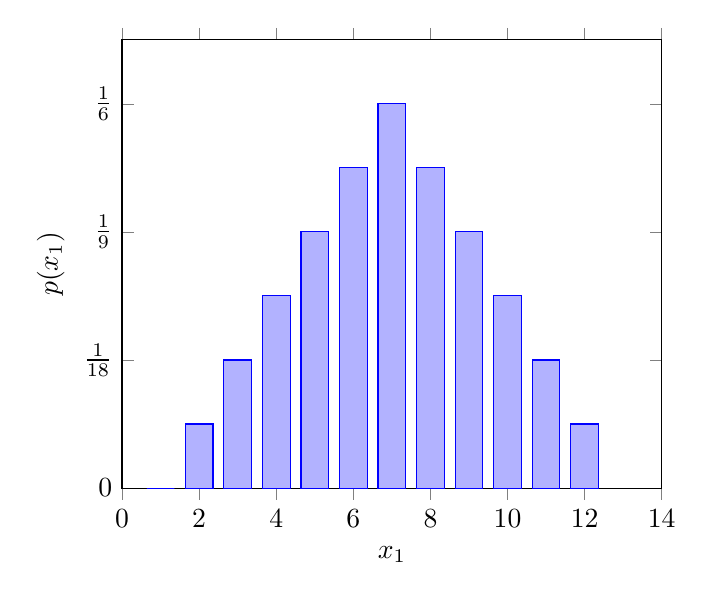
\begin{tikzpicture}
    \begin{axis}[
        ybar, 
        xmin = 0, 
        xmax = 14, 
        ymin = 0, 
        ymax = 7/36,
        yticklabel style={/pgf/number format/frac, /pgf/number format/frac shift=2}, 
        ytick={0, 2/36, 4/36, 6/36},
        xlabel={$x_1$}, 
        ylabel={$p(x_1)$}]
        \addplot coordinates {
            (1, 0)
            (2, 1/36)
            (3, 2/36)
            (4, 3/36)
            (5, 4/36)
            (6, 5/36)
            (7, 6/36)
            (8, 5/36)
            (9, 4/36)
            (10, 3/36)
            (11, 2/36)
            (12, 1/36)
        };
    \end{axis} 
\end{tikzpicture}
\end{center}
\begin{changebar}
    \begin{example}
        The probability mass function of a random variable $X$ is given by $p(i) = c\lambda^i/i!$, $i = 0, 1, \dots,$ where $\lambda$ is some positive value. Find \begin{enumerate}[label=(\alph*)]
            \item $P\left\{ X = 0 \right\}$.
            \item $P\left\{ X > 2 \right\}$.
        \end{enumerate}
    \end{example}
    \begin{solution}
        Since $\displaystyle \sum^\infty_{i = 0} p(i) = 1$, we have \[
            c \sum^\infty_{i = 0} \frac{\lambda^i}{i!} = 1.    
        \] Because $\displaystyle e^x = \sum^\infty_{i = 0} \frac{x^i}{i!}$, this implies that \[
            ce^\lambda = 1 \text{ or } c = e^{-\lambda}.    
        \]
        Thus, we have: \begin{enumerate}[label=(\alph*)]
            \item $P\left\{ X = 0 \right\} = p(0) = e^{-\lambda}\lambda^0/0! = e^{-\lambda}$
            \item \[
                \begin{aligned}
                    P\left\{ X > 2 \right\} &= 1 - P\left\{ X \leq 2 \right\} \\
                    &= 1 - P\left\{ X = 0 \right\} - P\left\{ X = 1 \right\} - P\left\{ X = 2 \right\} \\
                    &= 1 - e^{-\lambda} - \lambda e^{-\lambda} - \frac{\lambda^2e^{-\lambda}}{2}.
                \end{aligned}    
            \]
        \end{enumerate}
    \end{solution}
\end{changebar}

We can see that the distribution function $F$ can be expressed in terms of $p(a)$ by \[
    F(a) = \sum_{\text{all $x \leq a$}} p(x).    
\] If $X$ is a discrete random variable whose possible values are $x_1, x_2, x_3, \dots$, where $x_1 < x_2 < x_3 < \dots$, then $F$ is a step function; that is, the value of $F$ is constant in the intervals $(x_{i-1}, x_i)$, then takes a step (or jump) of size $p(x_i)$ at $x_i$. For example, if $X$ has a probability mass function given by \[
    p(1) = \frac{1}{4},\, p(2) = \frac{1}{2},\, p(3) = \frac{1}{8},\, p(4) = \frac{1}{8},
\] then its cumulative distribution function is \[
    \begin{cases}
        0 & a < 1 \\
        \frac{1}{4} & 1 \leq a < 2 \\
        \frac{3}{4} & 2 \leq a < 3 \\
        \frac{7}{8} & 3 \leq a < 4 \\
        1 & 4 \leq a
    \end{cases}
\]
\pagebreak
\subsection{Expected value}
\begin{bdef}{Expected value}\label{expectedvalue}
    If $X$ is a discrete random variable having a probability mass function $p(x)$, then the \textbf{expectation}, or \textbf{expected value}, of $X$, denoted $E\left[ X \right]$, is defined by \[
        E\left[ X \right] = \sum_{x:\, p(x) > 0} xp(x).    
    \] In other words, the expected value of $X$ is a weighted average of the possible values that $X$ can assume, weighted by the probability that $X$ assumes it.
\end{bdef}
This definition of expectation is partly motivated by the frequency interpretation of probabilities. This assumes that if an infinite sequence of independent replications of an experiment is performed, then, for any event $E$, the proportion of time that $E$ occurs will be $P(E)$. Consider a random variable $X$ that must taken on one of the values $x_1, x_2, \dots, x_n$, with respective probabilities $p(x_1), p(x_2), \dots, p(x_n)$, and think of $X$ as representing our winnings in a single game of chance. That is, with probability $p(x_i)$, we shall win $x_i$ units. By the frequency interpretation, if we play this game continually, then the proportion of time that we win $x_i$ will be $p(x_i)$. Since this is true for all $i$, $i = 1, 2, \dots, n$, it follows that our average winnings per game will be \[
    \sum^n_{i = 1} x_ip(x_i) = E\left[ X \right].
\]
\begin{changebar}
    \begin{example}\label{dieexpected}
        Find $E\left[ X \right]$, where $X$ is the outcome when we roll a fair die.
    \end{example}
    \begin{solution}
        Since $p(1) = p(2) = p(3) = p(4) = p(5) = p(6) = \frac{1}{6}$, we obtain \[
            E\left[ X \right] = 1\left( \frac{1}{6} \right) + 2\left( \frac{1}{6} \right) + 3\left( \frac{1}{6} \right) + 4\left( \frac{1}{6} \right) + 5\left( \frac{1}{6} \right) + 6\left( \frac{1}{6} \right) = \frac{7}{2}.    
        \]
    \end{solution}
\end{changebar}
\begin{changebar}
    \begin{example}
        A contestant on a quiz show is presented with two questions, questions 1 and 2, which he is to attempt to answer in some order he chooses. If he decides to try question $i$ first, then he will be allowed to go on to question $j$, $j \neq i$, only if his answer to question $i$ is correct. If his initial answer is incorrect, he is not allowed to answer the other question. The question is to receive $V_i$ if he answers question $i$ correctly, $i = 1, 2$. For instance, he will receive $V_1 + V_2$ dollars if he answers both correctly. If the probability that he knows the answer to question $i$ is $P_i$, $i = 1, 2$, which question should he attempt to answer first so as to maximize his expected winnings? Assume that the events $E_i$, $i = 1, 2$ that he knows the answer to question $i$ are independent events.
    \end{example}
    \begin{solution}
        If he attempts to answer question 1 first, then he will win \[
            \begin{aligned}
                0 & \text{ with probability } & 1 - P_1 \\
                V_1 & \text{ with probability } & P_1(1-P_2) \\
                V_1 + V_2 & \text{ with probability } & P_1P_2
            \end{aligned}
        \] Thus, his expected winnings in this case will be \[
            V_1P_1(1-P_2) + (V_1 + V_2)P_1P_2    
        \] On the other hand, if he attempts to answer question 2 first, then he will win \[
            \begin{aligned}
                0 & \text{ with probability } & 1 - P_2 \\
                V_2 & \text{ with probability } & P_2(1 - P_1) \\
                V_1 + V_2 & \text{ with probability } & P_1P_2
            \end{aligned}    
        \] with expected winnings \[
            V_2P_2(1 - P_1) + (V_1 + V_2)P_1P_2.    
        \] Thus he should try question 1 first if \[
            V_1P_1(1 - P_2) \geq V_2P_2(1 - P_1)    
        \] or, equivalently, \[
            \frac{V_1P_1}{1 - P_1} \geq \frac{V_2P_2}{1 - P_2}.    
        \]
    \end{solution}
\end{changebar}

\pagebreak
\subsection{Expectation of a function of a random variable}
Suppose that we are given a discrete random variable $X$ along with its probability mass function and that we want to compute the expected value of some function of $X$, say $g(X)$. One method is that since $g(X)$ is itself a discrete random variable, it has a probability mass function which can in turn be derived from the probability mass function of $X$; once determined, we can compute $E\left[ g(x) \right]$ as usual.
\begin{changebar}
    \begin{example}
        Let $X$ denote a random variable that takes on any of the values $-1$, $0$, and $1$ with respective probabilities \[
            P\left\{ X = -1 \right\} = 0.2 \: P\left\{ X = 0 \right\} = 0.5 \: P\left\{ X = 1 \right\} = 0.3.    
        \]
        Compute $E\left[ X^2 \right]$.
    \end{example}
    \begin{solution}
        Let $Y = X^2$. Then the probability mass function of $Y$ is given by \[
            \begin{aligned}
                P\left\{ Y = 1 \right\} &= P\left\{ X = -1 \right\} + P\left\{ X = 1 \right\} &= 0.5 \\
                P\left\{ Y = 0 \right\} &= P\left\{ X = 0 \right\} &= 0.5
            \end{aligned}    
        \]
    \end{solution}
\end{changebar}
\begin{bdef}{Expected value of $g(X)$}\label{expectedvaluegx}
    If $X$ is a discrete random variable that takes on one of the values $x_i$, $i \geq 1$, with respective probabilities $p(x_i)$, then, for any real-valued function $g$, \[
        E\left[ g(X) \right] = \sum_i g(x_i)p(x_i).    
    \]
\end{bdef}
\begin{changebar}
    \begin{example}[Utility]
        Suppose that you must choose one of two possible actions, each of which can result in any of $n$ consequences, denoted as $C_1, \dots, C_n$. Suppose that if the first action is chosen, then consequence $C_i$ will result with probability $p_i$, $i = 1, \dots, n$, whereas if the second action is chosen, then consequence $C_i$ will result with probability $q_i$, $i = 1, \dots, n$, where \[
            \sum^n_{i = 1} p_i = \sum^n_{i = 1} q_i = 1.    
        \] The following approach can be used to determine which action to choose: \begin{itemize}
            \item Start by assigning numerical values to the different consequences: identify the most and least desirable consequences; call them $C$ and $c$, respectively, and assign them the values $1$ and $0$, respecttively.
            \item Now consider any of the remaining $n - 2$ consequences, say $C_i$. To value this consequence, imagine that you are given the choice between either receiving $C_i$ or taking part in a random experiment that either earns you consequence $C$ with probability $u$ or consequence $c$ with probability $1 - u$. 
            \item Clearly your choice depends on the value of $u$ -- that is, there is a value of $u$ at which you are indifferent between either receiving $C_i$ or participating in the experiment that could result in either $C$ or $c$, below which the risk of receiving consequence is too great, and above which the chance of receiving $C$ is too great to justify participating in the experiment.
            \item This value of indifference $u$ is termed the \textbf{utility} of $C_i$, and we will denote it $u(C_i)$.
            \item To determine which action is superior, we evaluate them both in turn, starting with the first one, which results in consequence $C_i$ with probability $p_i$. We can imagine selecting a random value $i$ from $1$ to $n$ according to the probabilities $p_1, \dots, p_n$; if value $i$ is chosen, you receive consequence $C_i$. 
            \item However, since the value of $C_i$ is by definition equivalent to obtaining consequence $C$ with probability $u(C_i)$ or consequence $c$ with probability $1 - u(C_i)$, then we can imagine the outcome of selecting the first action as having a probability of being consequence $C$ of \[
                \sum^n_{i = 1} p(i)u(C_i).
            \]
            \item Similarly, the selecting the second action would have a probability of resulting in consequence $C$ with probability \[
                \sum^n_{i = 1} q(i)u(C_i).    
            \]
            \item Since $C$ is preferable to $c$, it follows that the action which is preferable is that which has a greater expected value calculated in this way.
            \item According to this decision-making strategy, the worth of an action can be measured by the expected value of the utility of its consequence, and the action with the largest expected utility is the most preferable.
        \end{itemize}
    \end{example}
\end{changebar}
\begin{bdef}{Moments of $X$}\label{moments}
    The expected value $E\left[ X \right]$ of a random variable $X$ is also referred to as the \textbf{mean} or the \textbf{first moment} of $X$. The quantity $E\left[ X^n \right], n \geq 1$, is called the \textbf{$n$th moment of $X$}. By \nameref{expectedvaluegx}, \[
        E\left[ X^n \right] = \sum_{x:\: p(x) > 0} x^np(x)
    \]
\end{bdef}

\pagebreak
\subsection{Variance}
\begin{bdef}{Variance}\label{variance}
    If $X$ is a random variable with mean $\mu$, then the \textbf{variance} of $X$, denoted $\Var(X)$, is defined by \[
        \Var(X) = E\left[ (X - \mu)^2 \right].    
    \] An alternate formula, derived below, is \[
        \Var(X) = E\left[ X^2 \right] - \left( E\left[ X \right] \right)^2.    
    \] Because $\Var(X)$ is the sum of nonnegative terms, it follows that $\Var(X) \geq 0$ and thus \[
        E\left[ X^2 \right] \geq \left( E\left[ X \right] \right)^2.    
    \]
\end{bdef}
\[
    \begin{aligned}
        \Var(X) &= E\left[ (X - \mu)^2 \right] \\
        &= \sum_x (x - \mu)^2p(x) \\
        &= \sum_x (x^2 - 2\mu x + \mu^2)p(x) \\
        &= \sum_x x^2p(x) - 2\mu\sum_x xp(x) + \mu^2\sum_x p(x) \\
        &= E\left[ x^2 \right] - 2\mu^2 + \mu^2 \\
        &= E\left[ x^2 \right] - \mu^2 \\
        &= E\left[ x^2 \right] - \left( E\left[ X \right] \right)^2
    \end{aligned}    
\]
\begin{changebar}
    \begin{example}
        Calculate $\Var(X)$ if $X$ represents the outcome when a fair die is rolled.
    \end{example}
    \begin{solution}
        From \autoref{dieexpected}, we know that $\mu = E\left[ X \right] = \frac{7}{2}.$ We then find $E\left[ X^2 \right]$: \[
            \begin{aligned}
                E\left[ X^2 \right] &= 1^2\left( \frac{1}{6} \right) + 2^2\left( \frac{1}{6} \right) + 3^2\left( \frac{1}{6} \right) + 4^2\left( \frac{1}{6} \right) + 5^2\left( \frac{1}{6} \right) + 6^2\left( \frac{1}{6} \right) \\
                &= \left( \frac{1}{6} \right)\left( 91 \right)
            \end{aligned}    
        \] Then \[
            \Var(X) = E\left[ X^2 \right] - \mu^2 = \frac{91}{6} - \left( \frac{7}{2} \right)^2 = \frac{35}{12}.     
        \]
    \end{solution}
\end{changebar}
\begin{changebar}
    \begin{example}[The friendship paradox]
        The friendship paradox is often expressed as saying that, on average, your friends have more friends than you do. More formally, suppose that there are $n$ people in a certain population, labeled $1, 2, \dots, n$, and that certain pairs of these individuals are friends. Let $f(i)$ denote the number of friends of person $i$ and let $f = \sum^n_{i = 1} f(i)$.

        Now, let $X$ be a randomly chosen individual, equally likely to be any of $1, 2, \dots, n$. That is, $p(i) = 1/n$, $i = 1, \dots, n$. Letting $g(i) = f(i)$ in \nameref{expectedvaluegx}, it follows that $E\left[ f(X) \right]$, the expected number of friends of $X$, is \[
            E\left[ f(X) \right] = \sum^n_{i = 1} f(i)p(i) = \sum^n_{i = 1} f(i)/n = f/n.    
        \] Also, letting $g(i) = f^2(i)$, it follows that $E\left[ f^2(X) \right]$ is \[
            E\left[ f^2(X) \right] = \sum^n_{i = 1} f^2(i)p(i) = \sum^n_{i = 1} f^2(i)/n.    
        \] Now suppose that each of the $n$ individuals writes down all the names of their friends, with each name written on a separate sheet of paper. Thus, each individual uses $f(i)$ sheets of paper for a total of $\sum^n_{i = 1} f(i) = f$ sheets. Now choose one of those sheets at random and let $Y$ denote the name written on that sheet. Let us compute $E\left[ f(Y) \right]$, the expected number of friends of the person whose name is on the chosen sheet. Because person $i$ has $f(i)$ friends, it follows that $i$ is on $f(i)$ of the sheets -- thus $i$ is the name on the chosen sheet with probability $\frac{f(i)}{f}$, $i = 1, \dots, n$. Consequently, \[
            E\left[ f(Y) \right] = \sum^n_{i = 1} f(i)\frac{f(i)}{f} = \sum^n_{i = 1} f^2(i)/f.    
        \] Using the two expected values calculated earlier, we see that \[
            E\left[ f(Y) \right] = \frac{E\left[ f^2(X) \right]}{E\left[ f(X) \right]} \geq E\left[ f(X) \right],    
        \] where the inequality follows from the fact that $E\left[ f^2(X) \right] \geq \left(E\left[ f(X) \right]\right)^2$. Thus $E\left[ f(X) \right] \leq E\left[ f(Y) \right]$ tells us that the number of friends of a randomly chosen individual is less than (or equal to, if everyone has the same amount of friends) the average number of friends of a randomly chosen friend.
        
        \begin{remark}
            The intuitive explanation is that $X$ is equally likely to be any of the individuals, but $Y$ is chosen with a probability proportional to how many friends an individual has -- thus the value of $Y$ is more likely to be a person with, on average, more friends than a randomly chosen individual.
        \end{remark}
    \end{example}
\end{changebar}

\begin{bdef}{Useful expected value and variance identities}\label{varianceident}
    For constants $a$ and $b$, \[
        E\left[ aX + b \right] = aE\left[ X \right] + b   
    \] \[
        \Var(aX + b) = a^2\Var(X)
    \]
\end{bdef}
\begin{bdef}{Standard deviation}\label{standarddeviation}
    The square root of $\Var(X)$ is called the \textbf{standard deviation} of $X$, denoted $\SD(X)$: \[
        \SD(X) = \sqrt{\Var(X)}    
    \]
\end{bdef}

\pagebreak
\subsection{Bernoulli and binomial random variables}
\begin{bdef}{Bernoulli random variables}\label{bernoullirandom}
    A random variable $X$ is said to be a \textbf{Bernoulli random variable} if its probability mass function is given by \[
        \begin{aligned}
            P\left\{ X = 0 \right\} &= 1 - p \\
            P\left\{ X = 1 \right\} &= p
        \end{aligned}    
    \] for some $p \in \left( 0, 1 \right)$.
\end{bdef}
\begin{bdef}{Binomial random variables}\label{binomialrandom}
    Suppose that $n$ independent trials of an experient, each of which results in a success with probability $p$ or in a failure with probability $1 - p$, are to be performed. If $X$ represents the number of successes that occur in the $n$ trials, then $X$ is said to be a \textbf{binomial random variable} with parameters $(n, p)$. Thus, a Bernoulli random variable is just a binomial random variable with parameters $(1, p)$.

    The probability mass function of a binomial random variable with parameters $(n, p)$ is given by \[
        p(i) = \binom{n}{i}p^i(1 - p)^{n - i},\, i = 0, 1, \dots, n    
    \]
\end{bdef}
The validity of the formula in \nameref{binomialrandom} can be verified by first observing that the probability of any particular sequence of $n$ outcomes containing $i$ successes and $n - i$ failures is, by the assumed independence of trials, $p^i(1 - p)^{n - i}$. Since there are $\binom{n}{i}$ different sequences of the $n$ outcomes leading to $i$ successes and $n - i$ failures, the formula follows.

Note that by \nameref{bth}, the probabilities sum to 1: that is, \[
    \sum^n_{i = 0} p(i) = \sum^n_{i = 0} \binom{n}{i}p^i(1 - p)^{n - i} = \left[ p + (1 - p) \right]^n = 1.    
\]
\begin{changebar}
    \begin{example}
        Consider a jury trial in which it takes 8 of the 12 jurors to convict the defendant. If we assume that the jurors act independently and that whether or not the defendant is guilty, each makes the right decision with probability $\theta$, what is the probability that the jury renders a correct decision if the defendant is guilty with a probability of $\alpha$?
    \end{example}
    \begin{solution}
        If the defendent is guilty, the probability of a correct decision is \[
            \sum_{i = 8}^{12} \binom{12}{i} \theta^i(1 - \theta)^{12 - i}    
        \] and if they are innocent, then the probability of a correct decision is \[
            \sum_{i = 5}^{12} \binom{12}{i} \theta^i(1 - \theta)^{12 - i}.    
        \] Then by conditioning on whether or not the defendant is guilty, the probability of making a correct decision is \[
            \alpha\sum^{12}_{i = 8} \binom{12}{i} \theta^i(1 - \theta)^{12 - i} + (1 - \alpha)\sum_{i = 5}^{12} \binom{12}{i} \theta^i(1 - \theta)^{12 - i}.    
        \]
    \end{solution}
\end{changebar}

\subsubsection{Properties of binomial random variables}
For a binomial random variable $X$ with parameters $n$ and $p$, note that \[
    \begin{aligned}
        E\left[ X^k \right] &= \sum^n_{i = 0} i^k \binom{n}{i}p^i(1 - p)^{n - i} \\
        &= \sum^n_{i = 1} i^k \binom{n}{i}p^i(1 - p)^{n - i}.
    \end{aligned} 
\] Using the identity \[
    i\binom{n}{i} = n\binom{n-1}{i-1}    
\] gives us \[
    \begin{aligned}
        E\left[ X^k \right] &= np \sum^n_{i = 0} i^{k - 1}\binom{n - 1}{i - 1}p^{i - 1}(1 - p)^{n - i} \\
        &= np \sum^{n - 1}_{j = 0} (j + 1)^{k - 1}\binom{n - 1}{j}p^j(1 - p)^{n - 1 - j} \\
        &= npE\left[ (Y + 1)^{k - 1} \right],
    \end{aligned}    
\] where $Y$ is a binomial random variable with parameters $n - 1, p$. The second line works by substituting $j$ for $i - 1$. By setting $k = 1$, we obtain \[
    E\left[ X \right] = np,    
\] and by setting $k = 2$, we obtain \[
    \begin{aligned}
        E\left[ X^2 \right] &= npE\left[ Y + 1 \right] \\
        &= np\left( E\left[ Y \right] + 1 \right) \\
        &= np\left[ (n-1)p + 1 \right]
    \end{aligned}.
\] Then \[
    \begin{aligned}
        \Var(X) &= E\left[ X^2 \right] - \left( E\left[ X \right] \right)^2 \\
        &= np\left[ (n-1)p + 1 \right] - (np)^2 \\
        &= np(1 - p).
    \end{aligned}    
\]
\begin{bdef}{Expected value and variance of binomial random variables}\label{expectedvaluebinomial}
    For a binomial random variable $X$ with parameters $n$ and $p$, \[
        \begin{aligned}
            E\left[ X \right] &= np \\
            \Var(X) &= np(1 - p).
        \end{aligned}
    \]
\end{bdef}
\begin{proposition}{Behavior of binomial probability mass function}
    If $X$ is a binomial random variable with parameters $(n, p)$ where $0 < p < 1$, then as $k$ goes from $0$ to $n$, $P\left\{ X = k \right\}$ first increases monotonically and then decreases monotonically, with a global maximum when $k = \left\lfloor (n + 1)p \right\rfloor$.
\end{proposition}

\subsubsection{Computing the binomial distribution function}

\pagebreak
\subsection{The Poisson random variable}

\subsubsection{Computing the Poisson distribution function}

\pagebreak
\subsection{Other discrete probability distributions}

\subsubsection{The geometric random variable}

\subsubsection{The negative binomial random variable}

\subsubsection{The hypergeometric random variable}

\subsubsection{The zeta (or Zipf) distribution}

\pagebreak
\subsection{Expected value of sums of random variables}

\pagebreak
\subsection{Properties of the cumulative distribution function}\label{cumdistproperties}
    \section{Index}
    \listoftheorems[ignoreall, show={definition}, title={List of Definitions}]
\end{document}